\documentclass[preprint,12pt]{elsarticle}

\journal{Computer Methods in Applied Mechanics and Engineering}

\usepackage[T1]{fontenc}
\usepackage[utf8]{inputenc}
\usepackage{hyperref}
\usepackage{url}
\usepackage{booktabs}
\usepackage{nicefrac}
\usepackage[protrusion=true,expansion=false]{microtype}
\usepackage{xcolor}
\usepackage{subcaption}
\usepackage{multirow}
\usepackage{amsmath,amssymb,amsfonts}
\usepackage{amsthm}
\usepackage{mathrsfs}
\usepackage{enumitem}
\usepackage{float}
\usepackage{algorithm}
\usepackage{algorithmicx}
\usepackage{algpseudocode}

\newtheorem{theorem}{Theorem} % continuous numbers
%%\newtheorem{theorem}{Theorem}[section] % sectionwise numbers
%% optional argument [theorem] produces theorem numbering sequence instead of independent numbers for Proposition
\newtheorem{proposition}[theorem]{Proposition}% 
\newtheorem{lemma}{Lemma}% 
%%\newtheorem{proposition}{Proposition} % to get separate numbers for theorem and proposition etc.

\newtheorem{example}{Example}
\newtheorem{remark}{Remark}

\newtheorem{definition}{Definition}
\newtheorem{assumption}{Assumption}

%%%

\newcommand{\R}{\mathbb{R}}
\newcommand{\cN}{\mathcal{N}}
\newcommand{\cL}{\mathcal{L}}
\newcommand{\cK}{\mathcal{K}}
\newcommand{\cD}{\mathcal{D}}
\newcommand{\cF}{\mathcal{F}}
\newcommand{\KL}{\mathrm{KL}}
\newcommand{\norm}[1]{\left\|#1\right\|_w}
\newcommand{\normsq}[1]{\left\|#1\right\|_w^{2}}
\newcommand{\ip}[2]{\langle #1,\, #2\rangle}
\newcommand{\hats}{\hat{s}}
\newcommand{\T}{\mathcal{T}}
\newcommand{\cG}{\mathcal{G}}


% frontmatter moved inside \begin{document}





\begin{document}

\begin{frontmatter}

\title{TEMPO: Regime-Aware Operator Learning with Locally Adapted POD Bases}

\author{Anonymous Authors}
\affiliation{organization={Anonymous Institution}}

\begin{abstract}
Operator learning methods approximate the solution map of a parametric PDE with a single global model, an assumption that fails when the governing parameter drives qualitatively distinct solution regimes.

We propose TEMPO, a framework that discovers latent regimes from unlabelled snapshots via Expectation-Maximization, fits a dedicated basis to each, and routes new inputs at inference time. The discovered partition captures both sources of solution variability: regime membership aligns with the shape of the initial condition across all parameter values, while the physical parameter shapes the dynamics within each regime. TEMPO(POD) outperforms the jointly-trained POD-DeepONet baseline by 13--50\% on 1D Burgers' equation and up to $5\times$ on 2D Darcy flow; per-parameter specialists fail catastrophically out-of-distribution.
\end{abstract}

\begin{highlights}
\item TEMPO discovers solution regimes from data and fits a dedicated basis to each.
\item Regime-local bases match or outperform a single global basis of the same rank.
\item TEMPO(POD) reduces error by 13--50\% on Burgers' and up to $4.75\times$ on Darcy flow.
\item TEMPO trains across all parameter values and handles multiple solution regimes.
\item Regime structure reflects initial conditions and physical parameters without labels.
\end{highlights}


\begin{keyword}
operator learning \sep parametric PDE \sep regime discovery \sep proper orthogonal decomposition \sep expectation-maximization \sep neural operator
\end{keyword}

\end{frontmatter}

\section{Introduction}\label{sec:intro}

Operator learning approximates the solution map of a parametric PDE from data,
enabling instant prediction without re-solving the governing equations at each
new parameter value~\cite{Kovachki2024}.
The dominant paradigm — exemplified by DeepONet~\cite{Lu2019} and
POD-DeepONet~\cite{Lu2022} — trains a single global model over the entire
parameter space.
This works well when solutions form a simple manifold, but breaks down when
the governing parameter drives \emph{qualitatively distinct} dynamics:
viscosity separating laminar flow from near-discontinuous shocks, or source
magnitude producing solutions that differ by orders of magnitude in amplitude.
When regimes differ fundamentally, a single global basis must split its capacity across all of them, fitting none well.

Several methods make the basis richer while still fitting a single model to all trajectories.
POD-PoU~\cite{Sharma2025} trains a partition-of-unity mixture of POD bases
with a shared branch, reducing error on sharp-gradient problems but without
discovering the underlying regime structure.
NeuralPOD~\cite{Mou2026} constructs nonlinear orthogonal basis functions via
greedy residual minimization, representing each mode as a neural network and
thus overcoming the linear subspace constraint.
Neither, however, provides a way to route a new input to the right representation at test time.

Clustering snapshots and fitting local bases to each cluster is a classical
idea in reduced-order modeling~\cite{Amsallem2012, Hess2019}.
Daniel et al.~\cite{Daniel2020} extend this to deep learning by clustering
solution subspaces on the Grassmann manifold and training a dictionary
selector at inference.
These methods assign each snapshot to a single cluster offline, with no feedback between the clustering and the operator being trained on top of it.

We propose \textbf{TEMPO} (\textit{Trajectory EM Mixture of POD Operators}),
which closes this gap in a principled probabilistic framework.
TEMPO models the trajectory ensemble as a Gaussian mixture and recovers regime
structure via Expectation-Maximization (EM): the E-step softly assigns each
trajectory to regimes based on reconstruction quality, while the M-step
rebuilds a dedicated NeuralPOD basis per regime — so as bases sharpen,
assignments improve, and vice versa.
After convergence, a GatingNet and per-regime BranchNets are trained jointly,
routing new inputs to the correct regime at inference.

\textbf{Contributions:}
\begin{itemize}[leftmargin=1.5em]
  \item \textbf{TEMPO framework.} A two-phase mixture-of-operators for
    parametric PDEs: an offline EM that discovers $M$ latent regimes from
    unlabelled snapshots and fits a dedicated orthogonal (POD) or nonlinear
    (NeuralPOD) basis to each; an online phase where a GatingNet and $M$
    BranchNets are trained with a KL penalty that anchors routing to the
    offline regime partition.

  \item \textbf{Adaptive basis update.} A distribution-shift criterion that
    monitors moment changes in regime composition across EM iterations and
    selects per-regime between full retraining, incremental mode
    addition/pruning, or skipping.

  \item \textbf{Theoretical guarantee.} Regime-local bases achieve
    reconstruction error no greater than the global rank-$K$ optimum for
    any soft-assignment matrix and any $M$, $K$
    (Proposition~\ref{prop:advantage}).

  \item \textbf{Experiments.} On 1D Burgers' and 2D Darcy flow, TEMPO(POD)
    reduces error by $13$--$50\%$ over the jointly-trained POD-DeepONet
    baseline, while per-parameter specialists fail badly out-of-distribution.
\end{itemize}


\section{Problem Statement}\label{sec:problem}

Let $\Omega \subset \R^d$ be a bounded spatial domain and $\T \subset \R_{\geq 0}$ a time interval.

We are given a dataset of $N$ solution trajectories:
\begin{equation}
  \cD = \bigl\{\,(u^{(i)}_0,\,\kappa^{(i)},\,s^{(i)})\,\bigr\}_{i=1}^{N},
  \qquad
  s^{(i)} = s\!\left(\cdot,\,\cdot\,;\,u^{(i)}_0,\kappa^{(i)}\right)
  \in L^2(\Omega\times\mathcal{T}),
  \label{eq:dataset}
\end{equation}
where $u_0^{(i)} \in \mathcal{U} = L^2(\Omega)$ is the initial condition and $\kappa^{(i)} \in \cK$ the physical parameter.
Each trajectory $s^{(i)}$ is discretized on $N_y = N_t N_x$ quadrature points
$\{y_j = (x_j, t_j),\, w_j\}_{j=1}^{N_y}$ covering the product grid
$\Omega \times \mathcal{T}$, with weighted norm $\|f\|_w^2 = \sum_j w_j f(y_j)^2$.

\begin{figure}[b]
  \centering
  
\includegraphics[width=0.45\textwidth]{TEMPO/main/figs/regimes_fig.png}
    \caption{Training dataset $\cD$: solution trajectories $s^{(i)}$ on
$\Omega\times\mathcal{T}$ for different $\kappa^{(i)}\in\cK$. Solutions
change character fundamentally across parameter values.}

  \label{fig:dataset}
\end{figure}

\begin{definition}[Solution operator]
\label{def:operator}
The \emph{solution operator}
 \[ \cG: \mathcal{U} \times \cK \to L^2(\Omega \times \T) \]
maps each pair $(u_0,\kappa)$ to the full space-time solution:
$\cG(u_0,\kappa) = s(\,\cdot\,,\,\cdot\,;\,u_0,\kappa)$.
\end{definition}


The operator $\cG$ is unknown and expensive to evaluate directly. The \emph{operator learning problem} is to construct $\hat{\cG} \approx \cG$ from $\cD$ alone, generalizing to unseen $(u_0,\kappa) \notin \cD$ without solving the PDE.


\paragraph{Multi-regime assumption}

When solutions change character fundamentally across $\cK$, the optimal low-dimensional representation differs from regime to regime, and no single global basis captures the full solution diversity. We formalize this observation via a latent variable model over the trajectory ensemble.

\begin{definition}[Generative model]
\label{def:generative}
Each trajectory arises from one of $M$ latent regimes. The regime label $z_i \in \{1,\ldots,M\}$ is unobserved and drawn from a categorical prior,
\begin{equation}
  z_i \sim \mathrm{Categorical}(\pi_1,\ldots,\pi_M),
  \qquad \pi_m \geq 0,\quad \textstyle\sum_m \pi_m = 1.
  \label{eq:prior}
\end{equation}
Conditioned on $z_i = m$, the trajectory is distributed as
\begin{equation}
 ( s^{(i)} \mid z_i{=}m) \;\sim\;
  \cN\!\bigl(\hats_m^{(i)},\;\sigma^2 W^{-1}\bigr),
  \label{eq:likelihood}
\end{equation}
where $W = \mathrm{diag}(w_1,\ldots,w_{N_y})$ is the quadrature weight matrix, $\sigma^2 > 0$ controls the softness of regime assignments, and $\hats_m^{(i)}$ is the regime-$m$ approximation to $s^{(i)}$.
\end{definition}


The generative model leaves $\hats_m^{(i)}$ unspecified. We require only that it admits a \emph{low-rank trajectory decomposition}:
\begin{equation}
  \hats_m^{(i)}(y)
  \;=\; \phi_0^{(m)}(y)
  + \sum_{k=1}^{K_m}
    \lambda_k^{(m,i)}\,\phi_k^{(m)}(y),
  \qquad y = (x,t) \in \Omega\times\mathcal{T},
  \label{eq:separable}
\end{equation}
where $\phi_k^{(m)} : \Omega\times\mathcal{T}\to\mathbb{R}$ are spatiotemporal
mode functions and $\lambda_k^{(m,i)} \in \mathbb{R}$ a scalar amplitude
for trajectory~$i$ on mode~$k$.
This form encompasses POD~\citep{Lu2022} and learned neural bases~\citep{Mou2026};
in this work we adopt the latter.

\begin{definition}[Regime approximator]
\label{def:approx}
The parameters of regime $m$ are
$\Phi_m = \{\phi_k^{(m)}\}_{k=0}^{K_m}$
and scalar amplitudes
$\Lambda_m = \{\lambda_k^{(m,i)}\}_{k=1,\,i=1}^{K_m,\,N}$,
where $\phi_0^{(m)} : \Omega\times\mathcal{T}\to\mathbb{R}$ is the regime mean field,
$\{\phi_k^{(m)}\}_{k \geq 1}$ spatiotemporal mode functions,
$\lambda_k^{(m,i)}\in\mathbb{R}$ the scalar amplitude of trajectory~$i$ on mode~$k$,
and $K_m \leq K_{\max}$ the adaptive mode count.
\end{definition}

The learning problem decomposes into two phases: discovering the latent regime structure from $\cD$ \emph{offline}, then training a deployable operator for fast inference \emph{online}.


\paragraph{Phase 1: Offline regime discovery}

Since the regime labels $z_i$ in~\eqref{eq:likelihood} are unobserved,
we recover the bases $\{\Phi_m\}$, mixture weights $\pi$, and noise
level $\sigma^2$ by maximizing the observed-data log-likelihood:
\begin{equation}
  (\Phi^*,\pi^*,\sigma^{2*})
  \;=\; \operatorname*{arg\,max}_{\Phi,\,\pi,\,\sigma^2}
  \;\sum_{i=1}^N \log \sum_{m=1}^M
    \frac{\pi_m\,\det(W)^{1/2}}{(2\pi\sigma^2)^{N_y/2}}
    \exp\!\!\left(-\frac{\normsq{s^{(i)}-\hats_m^{(i)}}}{2\sigma^2}\right).
  \label{eq:mle}
\end{equation}
The solution yields soft regime responsibilities
$\gamma_{im}^* = p(z_i{=}m \mid s^{(i)},\Phi^*,\pi^*,\sigma^{2*})$
that serve as supervision for Phase~2.



\paragraph{Phase 2: Online operator learning}

With bases $\{\Phi_m^*\}$ and responsibilities $\{\gamma_{im}^*\}$ frozen,
we train a gating network (\emph{GatingNet}) and $M$ branch networks (\emph{BranchNets}) that map a new input
$(u_0, \kappa)$ to a weighted combination of local regime predictions.
The precise architecture and loss are given in Section~\ref{sec:online}.
The quality of the final operator is measured by the mean relative $L^2$ error:
\begin{equation}
  \varepsilon \;=\; \frac{1}{N_\mathrm{test}}
  \sum_{i=1}^{N_\mathrm{test}}
  \frac{\norm{s^{(i)} - \hat{s}(\cdot;\,u_0^{(i)},\kappa^{(i)})}}
       {\norm{s^{(i)}}} .
  \label{eq:metric}
\end{equation}















\section{Method}\label{sec:method}



All methods studied in this work share a common two-phase structure:
an \emph{offline} basis-fitting phase that constructs a low-rank
approximation to the solution manifold from snapshots in $\mathcal{D}$,
and an \emph{online} operator-learning phase that trains a branch
network to predict expansion coefficients from a new input
$(u_0, \kappa)$.
The four methods differ along two independent axes:

\begin{itemize}
  \item \textbf{Basis type.}
    A \emph{linear} (POD) basis uses SVD of the (weighted) snapshot
    matrix; a \emph{nonlinear} (NeuralPOD) basis learns spatiotemporal
    mode networks by sequential residual minimization.
  \item \textbf{Number of regimes.}
    A \emph{single-regime} operator fits one global basis to all
    snapshots; a \emph{multi-regime} operator (TEMPO) discovers $M$
    latent regimes via EM and assigns a dedicated basis to each.
\end{itemize}

\noindent
This gives four combinations:
POD-DeepONet~\cite{Lu2022} (linear, global),
NeuralPOD-DeepONet (nonlinear, global, our extension of~\cite{Mou2026}),
TEMPO(POD) (linear, $M$ regimes), and
TEMPO(NeuralPOD) (nonlinear, $M$ regimes).

\subsection{Basis Representations}\label{sec:bases}


\subsubsection{POD Basis}

Let $\phi_0 := \bar{s} = \tfrac{1}{N}\sum_i s^{(i)}$ be the mean field
and $\tilde{S} \in \mathbb{R}^{N_y \times N}$ the matrix with columns
$\tilde{s}^{(i)} = s^{(i)} - \phi_0$.
The rank-$K$ truncated SVD $\tilde{S} \approx U_K \Sigma_K V_K^\top$
yields orthonormal modes $\{\phi_k\}_{k=1}^K$ (columns of $U_K$) and
coefficients $\lambda_k^{(i)} = [\Sigma_K V_K^\top]_{ki}$; the
approximation
\begin{equation}
  \hat{s}^{(i)} = \phi_0 + \sum_{k=1}^{K} \lambda_k^{(i)}\,\phi_k
  \label{eq:pod_approx}
\end{equation}
is optimal in the $L^2$ sense among all rank-$K$ affine representations.

For TEMPO(POD), the M-step~\eqref{eq:mstep_phi} is solved analytically:
set $\phi_0^{(m)} := \bar{s}_m = \frac{1}{N_m}\sum_i \gamma_{im} s^{(i)}$,
where $N_m = \sum_i \gamma_{im}$, and apply SVD to
the weighted centered matrix with columns
$\sqrt{\gamma_{im}}\,(s^{(i)}-\phi_0^{(m)})$.
This is the closed-form linear analogue of Algorithm~\ref{alg:npod}.

\subsubsection{NeuralPOD Basis}\label{sec:neuralpod_basis}

To overcome the linearity constraint, we parametrize each mode
function $\phi_k : \Omega{\times}\mathcal{T} \to \mathbb{R}$ as a
Fourier feature network~\cite{Tancik2020}; we call the resulting basis a \emph{Fourier NeuralPOD} basis:
\begin{equation}
  \phi_k(y) \;=\; f_{\theta_k}\!\bigl(\psi(y)\bigr),
  \qquad
  \psi(y) \;=\;
  \bigl[\sin(2\pi By),\;\cos(2\pi By)\bigr],
  \label{eq:ffn}
\end{equation}
where $B \in \mathbb{R}^{F \times d}$ is a fixed random matrix drawn
once at initialization and $f_{\theta_k} : \mathbb{R}^{2F} \to \mathbb{R}$
is a small MLP with Tanh activations.
Plain MLPs exhibit spectral bias~\cite{Rahaman2019}; the Fourier encoding
resolves this.
For multi-scale coverage, the rows of $B$ are partitioned evenly across
$L$ frequency scales $\sigma_1 < \cdots < \sigma_L$: the $\ell$-th block is drawn from
$\mathcal{N}(0,\,\sigma_\ell^2 I)$.
The mean field $\phi_0$ uses the same architecture.

The scalar amplitudes $\lambda_k^{(i)} \in \mathbb{R}$ are direct
learnable parameters, one per training trajectory, optimized jointly
with $\phi_k$.
After Phase~1 they are frozen and serve as regression targets for the
BranchNet in Phase~2.

Modes are learned by \emph{greedy residual minimization}~\cite{Mou2026}.
Let $r^{(0,i)} = s^{(i)} - \phi_0$, where $\phi_0$ is fitted to the snapshot mean $\bar{s}$ defined above.
For each subsequent mode $k \ge 1$, given the residual
\begin{equation}
  r^{(k-1,i)}(y)
  = s^{(i)}(y)
  - \phi_0(y)
  - \sum_{\ell=1}^{k-1}\lambda_\ell^{(i)}\,\phi_\ell(y),
  \label{eq:residual_global}
\end{equation}
we solve
\begin{equation}
  \min_{\phi_k,\,\{\lambda_k^{(i)}\}}
  \sum_{i=1}^{N} \sum_j w_j
  \Bigl(\lambda_k^{(i)}\,\phi_k(y_j) - r_j^{(k-1,i)}\Bigr)^{\!2}
  \label{eq:neuralpod_loss}
\end{equation}
(the global case with uniform weights; the $\gamma$-weighted
generalization used in TEMPO is Algorithm~\ref{alg:npod}).
Mode addition stops when the residual falls below fraction $\tau$ of
the initial variance,
\begin{equation}
  \sum_{i=1}^N \|r^{(k,i)}\|_w^2
  \;<\;
  \tau \cdot \sum_{i=1}^N \|s^{(i)} - \bar{s}\|_w^2,
  \label{eq:npod_tol}
\end{equation}
or $k = K_{\max}$.
Each mode captures the largest remaining variance component — the nonlinear analogue of Gram--Schmidt orthogonalization.

\subsection{Single-Regime Operators}\label{sec:single}


\subsubsection{POD-DeepONet}

POD-DeepONet~\cite{Lu2022} replaces the learned trunk network of
DeepONet~\cite{Lu2019} with the fixed POD basis.
After computing the global modes $\{\phi_k\}_{k=1}^K$ and training
coefficients $\{\lambda^{(i)}\}$ offline, a branch network
$\mathcal{B}_\theta : \mathbb{R}^{m_s + d_\kappa} \to \mathbb{R}^K$
is trained online by regression against these coefficients:
\begin{equation}
  \mathcal{L}_{\mathrm{branch}}
  = \frac{1}{N}\sum_{i=1}^{N}
    \bigl\|\mathcal{B}_\theta(u_0^{(i)},\,\kappa^{(i)})
    - \lambda^{(i)}\bigr\|^2.
  \label{eq:pod_branch_loss}
\end{equation}
The prediction at any $(x,t) \in \Omega \times \mathcal{T}$ is
\begin{equation}
  \hat{s}(x,t;\,u_0,\kappa)
  = \phi_0(x,t)
  + \sum_{k=1}^{K}
    \mathcal{B}_{\theta,k}(u_0,\kappa)\,\phi_k(x,t).
  \label{eq:pod_predict}
\end{equation}

\subsubsection{NeuralPOD-DeepONet}\label{sec:neuralpod_deeponet}

Mou et al.~\cite{Mou2026} introduce NeuralPOD and pair it with a
DeepONet branch network to predict mode coefficients for unseen inputs.
We adopt this combination, which we refer to as \emph{NeuralPOD-DeepONet},
as a single-regime baseline and as the per-regime basis learner within TEMPO(NeuralPOD).

The procedure follows POD-DeepONet exactly with the Fourier NeuralPOD basis substituted for POD.
Offline fitting yields coefficients $\boldsymbol{\lambda}^{(i)} \in \mathbb{R}^K$; online, a branch network minimizes~\eqref{eq:pod_branch_loss} and prediction follows~\eqref{eq:pod_predict}.
At equal mode count $K$, the nonlinear basis spans a strictly richer function space than POD.


\subsection{TEMPO: Offline Regime Discovery}\label{sec:offline}


A single global basis — whether linear or nonlinear — must compromise
between qualitatively distinct regimes, as the optimal basis geometry
differs fundamentally between them.
TEMPO avoids this by constructing a dedicated basis for each of $M$
latent regimes, discovered from unlabelled trajectories via EM on
the generative model of Definition~\ref{def:generative}.

\paragraph{Initialization}
A global POD is computed on all $N$ trajectories; each trajectory is
projected to a $d_0$-dimensional coefficient vector
$\alpha^{(i)} \in \mathbb{R}^{d_0}$.
Running a standard GMM on $\{\alpha^{(i)}\}$ yields initial
responsibilities $\gamma_{im}^{(0)}$, weights $\pi_m^{(0)}$,
and per-regime statistics $(\mu_m^{(0)}, \Sigma_m^{(0)})$.
Each regime basis $\Phi_m^{(0)}$ is then fitted to the
responsibility-weighted ensemble: for TEMPO(NeuralPOD) via
\textsc{NeuralBasis} (Algorithm~\ref{alg:npod}); for TEMPO(POD)
via the weighted SVD of Section~\ref{sec:bases}.
The noise level $\sigma^2$ is calibrated from the initial
reconstructions rather than treated as a free hyperparameter:
\begin{equation}
  \sigma^2 \;\leftarrow\;
  \frac{1}{2N}\sum_{i=1}^N\sum_{m=1}^M
  \gamma_{im}^{(0)}\,\bigl\|s^{(i)} - \hat{s}_m^{(i)}\bigr\|_w^2,
  \label{eq:sigma2_calib}
\end{equation}
$\sigma^2$ is held fixed throughout EM; improving bases reduce residuals,
which progressively sharpens regime assignments.

\paragraph{E-step}
At iteration $q$, the responsibility of trajectory $i$ for regime $m$
is updated by Bayes' rule on the Gaussian likelihood~\eqref{eq:likelihood}:
\begin{equation}
  \gamma_{im}^{(q)}
  = \frac{
    \pi_m^{(q-1)}\,
    \exp\!\Bigl(-\dfrac{\|s^{(i)}-\hat{s}_m^{(i)}\|_w^2}{2\sigma^2}\Bigr)
  }{
    \sum_{j=1}^{M}
    \pi_j^{(q-1)}\,
    \exp\!\Bigl(-\dfrac{\|s^{(i)}-\hat{s}_j^{(i)}\|_w^2}{2\sigma^2}\Bigr)
  },
  \label{eq:estep}
\end{equation}
where $\hat{s}_m^{(i)}$ is evaluated via~\eqref{eq:separable}
using $\Phi_m^{(q-1)}$ and $\Lambda_m^{(q-1)}$.
As the bases improve in the M-step, the reconstructions $\hat{s}_m^{(i)}$
sharpen and the E-step automatically refines regime assignments in response —
distinguishing TEMPO from a GMM applied to a fixed feature space.
When $\kappa$ drives large amplitude variation (as with $\beta\in[0.01,100]$
in the Darcy experiments), replacing the squared norm with the relative squared norm
$\|s^{(i)}-\hat{s}_m^{(i)}\|_w^2/\|s^{(i)}\|_w^2$ throughout --- in~\eqref{eq:estep},
\eqref{eq:sigma2_calib}, and~\eqref{eq:mstep_phi} --- keeps E- and M-steps consistent
under a heteroscedastic likelihood with noise variance proportional to $\|s^{(i)}\|_w^2$.
When $\kappa$ is observed, the GMM initialization can operate in $\log\kappa$
space, and an optional $\kappa$-prior term in the E-step anchors assignments
to the known parameter structure.

\paragraph{M-step}
With responsibilities fixed, the M-step gives a closed-form update
for the mixture weights,
\begin{equation}
  \pi_m^{(q)} \leftarrow \frac{N_m^{(q)}}{N},
  \qquad N_m^{(q)} = \sum_{i=1}^{N}\gamma_{im}^{(q)},
  \label{eq:mstep_pi}
\end{equation}
and a weighted reconstruction problem for each basis:
\begin{equation}
  \min_{\Phi_m,\,\Lambda_m}
  \sum_{i=1}^{N} \gamma_{im}^{(q)}\,\|s^{(i)} - \hat{s}_m^{(i)}\|_w^2,
  \label{eq:mstep_phi}
\end{equation}
solved by weighted SVD for TEMPO(POD) or
\textsc{NeuralBasis} (Algorithm~\ref{alg:npod}) for
TEMPO(NeuralPOD).
Since gradient descent solves the NeuralPOD subproblem without guaranteeing
global optimality, TEMPO is a Generalized EM algorithm~\cite{Neal1998},
which guarantees that the observed-data log-likelihood is non-decreasing
at every iteration.

\begin{proposition}[Regime Approximation Advantage]\label{prop:advantage}
For any $\{\gamma_{im}\}\geq 0$ with $\sum_m\gamma_{im}=1$, any $M\geq 1$, any $K\geq 1$:
\[
  \varepsilon_{\mathrm{TEMPO}}^K \;\leq\; \varepsilon_{\mathrm{global}}^K,
\]
where
\begin{align*}
  \varepsilon_{\mathrm{global}}^K &= \min_{\substack{P\,\mathrm{rank\text{-}}K\\\mu}}\sum_i\|(I{-}P)(s^{(i)}{-}\mu)\|_w^2, \\
  \varepsilon_{\mathrm{TEMPO}}^K  &= \sum_m\min_{\substack{P_m\,\mathrm{rank\text{-}}K\\\mu_m}}\sum_i\gamma_{im}\|(I{-}P_m)(s^{(i)}{-}\mu_m)\|_w^2
\end{align*}
are the global and regime-wise optimal rank-$K$ reconstruction errors.
Proof: Appendix~\ref{app:proof}.
\end{proposition}

\begin{remark}
Both $\varepsilon_{\mathrm{TEMPO}}^K$ and $\varepsilon_{\mathrm{global}}^K$ use exactly $K$ basis functions per sample at inference; TEMPO stores $M$ regime-specific bases of rank $K$ offline, but routes each sample through exactly one.
\end{remark}

\begin{figure}[!htbp]
\centering
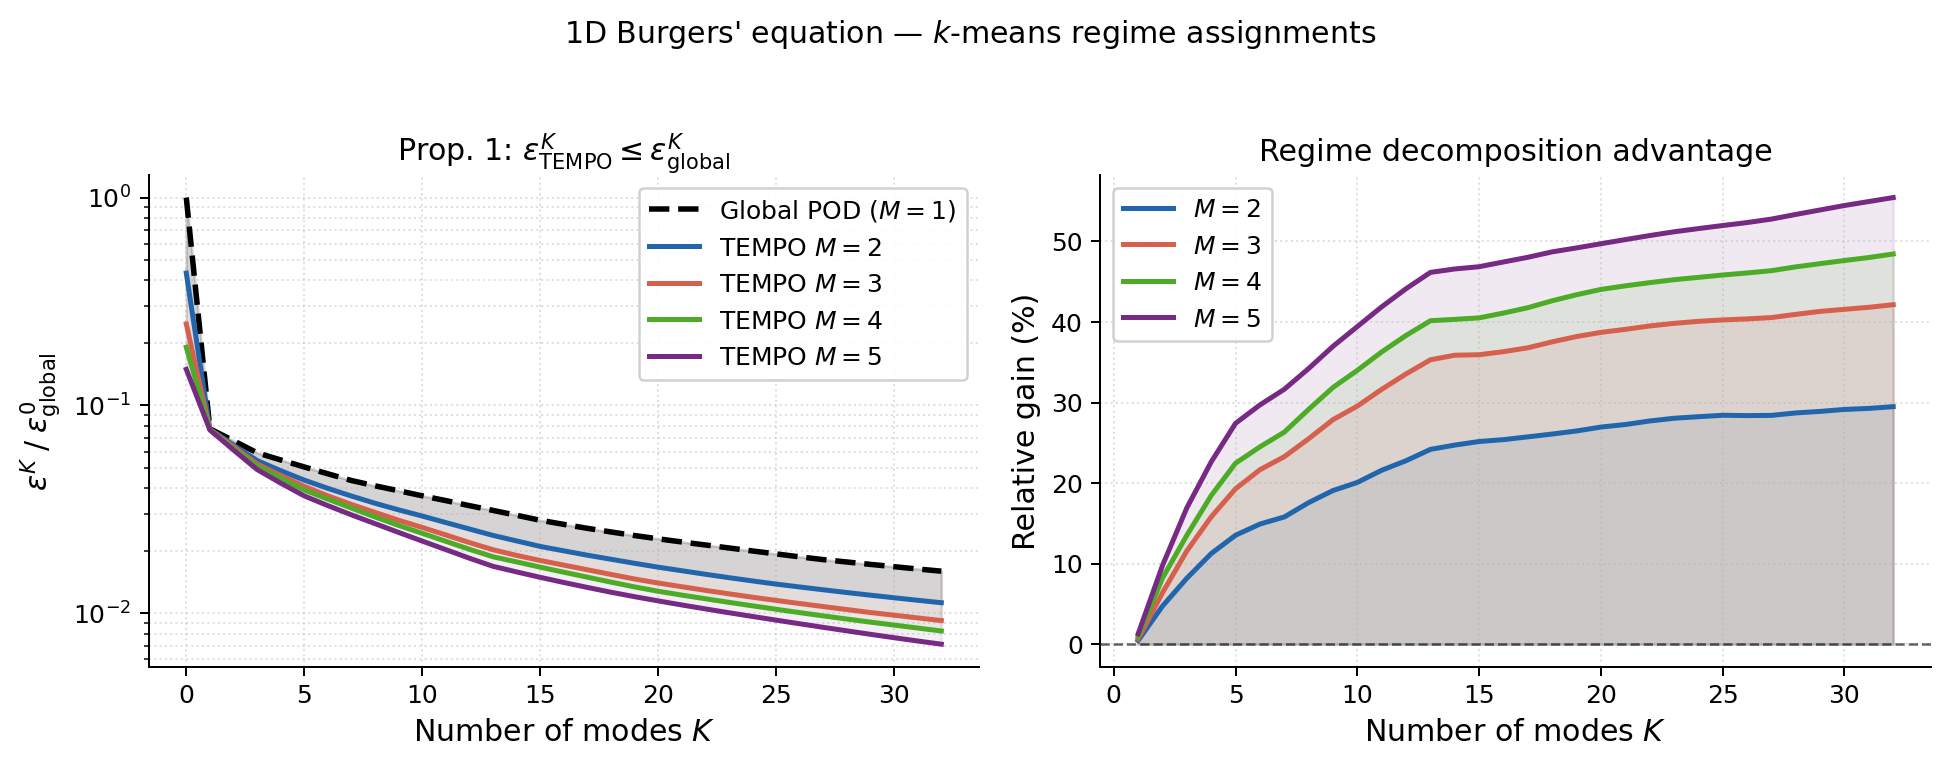
\includegraphics[width=\textwidth]{figs/theorem_verification.png}
\caption{Empirical verification of Proposition~\ref{prop:advantage} on 1D Burgers'.
  \textit{Left}: normalized reconstruction error (log scale); TEMPO lies strictly
  below the global POD for all $K\geq 1$.
  \textit{Right}: relative gain
  $(\varepsilon^K_{\mathrm{global}}-\varepsilon^K_{\mathrm{TEMPO}})/\varepsilon^K_{\mathrm{global}}$;
  all values are non-negative, with gains of $20$--$39\%$ at $K{=}10$.}
\label{fig:theorem}
\end{figure}

\paragraph{Adaptive basis update}
Retraining all $M$ NeuralPOD bases at every EM iteration is
computationally prohibitive.
We introduce a distribution-shift criterion to determine whether each
basis requires updating.
Let $\alpha^{(i)}$ denote the global POD projection of $s^{(i)}$,
computed once during initialization and fixed thereafter.
The responsibility-weighted first and second moments of regime $m$ are
\begin{align}
  \mu_m^{(q)}
  &= \frac{1}{N_m^{(q)}}\sum_{i=1}^N
    \gamma_{im}^{(q)}\,\alpha^{(i)},
  \label{eq:mu}\\
  \Sigma_m^{(q)}
  &= \frac{1}{N_m^{(q)}}\sum_{i=1}^N
    \gamma_{im}^{(q)}\,
    (\alpha^{(i)}-\mu_m^{(q)})(\alpha^{(i)}-\mu_m^{(q)})^\top.
  \label{eq:Sigma}
\end{align}
The distribution-shift criterion measures the relative change in these
moments between consecutive iterations:
\begin{equation}
  \Delta_m^{(q)}
  = \frac{\|\mu_m^{(q)} - \mu_m^{(q-1)}\|_2}
         {\|\mu_m^{(q-1)}\|_2 + \epsilon}
  + \frac{\|\Sigma_m^{(q)} - \Sigma_m^{(q-1)}\|_F}
         {\|\Sigma_m^{(q-1)}\|_F + \epsilon}.
  \label{eq:Delta}
\end{equation}
\noindent where $\epsilon > 0$ is a small numerical stabilizer.
$\Delta_m^{(q)}$ measures how much the composition of regime $m$ has changed,
not just the volume of reassignments.
Two trajectories with very different $\alpha^{(i)}$ swapping regimes
produce a large $\Delta_m^{(q)}$ and trigger a basis update;
two similar snapshots doing so do not.
Given thresholds $0 < \varepsilon_s < \varepsilon_l$, regime $m$ is
\textsc{Skip}ped if $\Delta_m^{(q)} < \varepsilon_s$, updated
\textsc{Incremental}ly (add or prune one mode) if
$\varepsilon_s \le \Delta_m^{(q)} < \varepsilon_l$, and fully retrained
from scratch (\textsc{Full rerun}) otherwise.
In the \textsc{Incremental} case, we compute the residual of the
current basis under the updated responsibilities $\gamma^{(q)}$, add
a new mode if $\sum_i \gamma_{im}^{(q)}\|r_m^{(K_m,i)}\|_w^2 \ge \tau\cdot\sum_i \gamma_{im}^{(q)}\|s^{(i)}-\bar{s}_m^{(q)}\|_w^2$,
and prune the last mode if its weighted contribution falls below
$\varepsilon_p$.
The \textsc{Full rerun} case uses a cold-start random initialization,
as warm-starting may trap gradient descent in the geometry of the previous regime.

\paragraph{Convergence and model selection}
The number of regimes $M$ is selected by two criteria: BIC on the EM log-likelihood
(penalizes complexity) and mean assignment entropy $H$. When they conflict, entropy
is decisive: a large gain $\Delta H$ from $M$ to $M{+}1$ signals a new regime.
EM terminates when $\max_m \Delta_m^{(q)} < \varepsilon_c$.
Selected values are $M{=}3$ (Burgers'), $M{=}4$ (Navier-Stokes), and $M{=}5$ (Darcy);
details for Burgers' are in Table~\ref{tab:regime_selection} (Appendix~\ref{app:exp}).
The complete offline procedure is given in Algorithm~\ref{alg:tempo}.

\subsection{TEMPO: Online Gated Operator}\label{sec:online}


After Algorithm~\ref{alg:tempo} converges, all regime bases
$\{\Phi_m^*\}$ and responsibilities $\{\gamma_{im}^*\}$ are frozen.
The online phase trains a GatingNet
$G: \mathbb{R}^{m_s + d_\kappa} \to \Delta^{M-1}$
that maps $(u_0, \kappa)$ to regime weights, and $M$ BranchNets
$\mathcal{B}_m: \mathbb{R}^{m_s + d_\kappa} \to \mathbb{R}^{K_m}$
that predict expansion coefficients for each regime.
The TEMPO prediction at query point $y = (x,t) \in \Omega\times\mathcal{T}$ is
\begin{equation}
  \hat{s}(y;\,u_0,\kappa)
  = \sum_{m=1}^{M} g_m(u_0,\kappa)
    \left[
      \phi_0^{(m)}\!(y)
      + \sum_{k=1}^{K_m}
        b_{m,k}(u_0,\kappa)\;
        \phi_k^{(m)}\!(y)
    \right],
  \label{eq:predict}
\end{equation}
where $\mathbf{g} = G(u_0,\kappa)$ and
$\mathbf{b}_m = \mathcal{B}_m(u_0,\kappa)$.
The BranchNet outputs $\mathbf{b}_m$ predict the expansion coefficients
$\boldsymbol{\lambda}_m^{(i)}$ for new inputs $(u_0,\kappa)$ not seen in training.
The prediction is mesh-free and evaluable at any $y\in\Omega\times\mathcal{T}$
without retraining.

\paragraph{Training objective}
Writing $g_m^{(i)} = g_m(u_0^{(i)},\kappa^{(i)})$, the online loss is
\begin{equation}
  \mathcal{L}_{\mathrm{online}}
  = \underbrace{
      \frac{1}{N}\sum_{i=1}^{N}
      \|s^{(i)} - \hat{s}(\cdot;\,u_0^{(i)},\kappa^{(i)})\|_w^2
    }_{\mathcal{L}_{\mathrm{data}}}
  +\;\eta_{\mathrm{KL}}
    \underbrace{
      \frac{1}{N}\sum_{i,m}
      g_m^{(i)}\log\frac{g_m^{(i)}}{\gamma_{im}^*}
    }_{\mathcal{L}_{\mathrm{KL}}}
  -\;\eta_{H}
    \underbrace{
      \frac{1}{N}\sum_{i,m}
      g_m^{(i)}\log g_m^{(i)}
    }_{-\mathcal{L}_{\mathrm{ent}}}.
  \label{eq:online_loss}
\end{equation}
$\mathcal{L}_{\mathrm{data}}$ drives reconstruction accuracy.
$\mathcal{L}_{\mathrm{KL}}$ anchors the online gating to the
offline regime partition: it penalizes deviation of $\mathbf{g}^{(i)}$
from the EM responsibilities $\boldsymbol{\gamma}_i^*$, so the
network cannot discard the discovered structure in pursuit of a
simpler routing.
$\mathcal{L}_{\mathrm{ent}}$ prevents collapse to a single expert,
ensuring all $M$ regime bases contribute.
The hyperparameters $\eta_{\mathrm{KL}}, \eta_H \ge 0$ trade
off these objectives.





\begin{figure}[H]
  \centering
  
\includegraphics[width=\textwidth]{TEMPO/main/figs/TEMPO_graphical_highlights_v2.png}
  \caption{\textbf{TEMPO pipeline} (illustrated on 1D Burgers').
    Offline: EM discovers $M$ regimes, each with a dedicated basis $\{\Phi_m\}$.
    Online: a GatingNet and $M$ BranchNets produce a weighted reconstruction.}
  \label{fig:pipeline}
\end{figure}

\section{Computational Experiments}
\label{sec:exp}

We evaluate TEMPO on parametric PDE benchmarks, verifying three claims:
(i)~the offline EM phase recovers interpretable, physics-consistent regime
structure from unlabelled snapshots;
(ii)~locally adapted bases achieve lower reconstruction error than a
single global basis at equal mode count;
(iii)~a gated operator with per-regime bases outperforms a single global basis when the data contains structured regimes.

\subsection{Experimental Setup}
\label{sec:setup}

\paragraph{Datasets}
We use three parametric PDE benchmarks; the first two are from PDEBench~\cite{Takamoto2022}.

\textbf{1D Burgers' equation.}
\begin{equation}
  u_t + u\,u_x = \nu\,u_{xx},
  \qquad x\in(-1,1),\quad t\in(0,2],
  \label{eq:burgers}
\end{equation}
with periodic boundary conditions and random initial conditions.
Viscosity $\nu\in\{0.001,\,0.01,\,0.1,\,1.0\}$ spans four qualitatively
distinct solution regimes: smooth diffusive profiles at $\nu{=}1.0$ and
near-discontinuous shock structures at $\nu{=}0.001$.
Each value provides $N{=}9{,}500$ trajectories on $N_x{=}1{,}024$
spatial points and $N_t{=}201$ time steps ($38{,}000$ total).

\textbf{2D Darcy flow.}
\begin{equation}
  -\nabla\cdot\bigl(a(x)\,\nabla u(x)\bigr) = \beta,
  \qquad x\in(0,1)^2,
  \label{eq:darcy}
\end{equation}
with zero Dirichlet boundary conditions.
Here $a(x)$ is a spatially varying permeability field sampled from a
random sum of Gaussians, and $\beta\in\{0.01,\,0.1,\,1.0,\,10.0,\,100.0\}$
is the constant source term.
Each value provides $N{=}8{,}000$ training and $1{,}000$ test samples
discretised on a $128{\times}128$ uniform grid ($N_y{=}16{,}384$ spatial points),
$40{,}000$ samples in total.
The operator maps $a(x)$ to the pressure solution $u(x)$; as a steady-state problem, $N_t{=}1$ and there is no time dependence.

\textbf{2D incompressible Navier-Stokes.}
\begin{equation}
  \partial_t \omega + \mathbf{u}\cdot\nabla\omega
  = \frac{1}{\mathrm{Re}}\,\Delta\omega + f,
  \qquad \mathbf{x}\in(0,1)^2,\; t\in(0,2],
  \label{eq:ns}
\end{equation}
with periodic boundary conditions, $\omega=\nabla\times\mathbf{u}$,
divergence-free $\mathbf{u}$ recovered via the stream function,
and Kolmogorov-type forcing
$f(\mathbf{x})=0.1\bigl(\sin 2\pi(x_1{+}x_2)+\cos 2\pi(x_1{+}x_2)\bigr)$~\citep{Li2021}.
Reynolds number $\mathrm{Re}\in\{100,\,1000,\,3600,\,10000\}$ spans four
qualitatively distinct regimes from smooth laminar flow to developed turbulence.
Each value provides $N{=}5{,}000$ trajectories on a $64{\times}64$ periodic
grid ($20{,}000$ total; $4{,}000$/$1{,}000$ train/test);
see Appendix~\ref{app:ns_data}.
Operator: $\mathbf{u}_0\mapsto(\mathbf{u}_t)_{t=1}^{20}$, $\Delta t{=}0.1$.

\paragraph{Methods}
We compare DeepONet~\cite{Lu2019}, POD-DeepONet~\cite{Lu2022},
FNO~\cite{Li2021}, and CNO~\cite{Raonic2023}—all trained jointly on all
parameter values via a single global model.
We introduce NeuralPOD-DeepONet (learned Fourier NeuralPOD basis with branch network);
TEMPO(POD) and TEMPO(NeuralPOD) (regime-aware bases discovered via EM, routed by
gating network). Per-parameter specialists serve as performance ceilings.
All methods implemented by the authors.
Evaluation: mean relative $L^2$ error~\eqref{eq:metric} per parameter value.
Inference times measured on a single NVIDIA RTX A5000 GPU, per sample.

%==========================================================================
\subsection{Main Results}
\label{sec:results}
%==========================================================================

\paragraph{1D Burgers' equation}
Table~\ref{tab:results} gives the cross-viscosity error matrix.
Per-$\nu$ specialists are unviable across the full range: a $\nu{=}0.1$
model degrades from $0.048$ to $0.461$ at $\nu{=}0.001$.
TEMPO(POD) addresses this by discovering regime structure jointly,
outperforming the joint POD-DeepONet baseline by 13--50\% across all~$\nu$.
TEMPO(NeuralPOD) does not surpass the joint baseline. NeuralPOD-DeepONet
already underperforms POD-DeepONet in the single-regime case ($0.229$
vs.\ $0.048$ at $\nu{=}0.1$): the branch network finds NeuralPOD coefficients
harder to predict than POD projections. In TEMPO this is amplified: each EM
iteration fits $M$ NeuralPOD bases from scratch, and errors in early
iterations feed back through the responsibilities into later ones.

\paragraph{2D Darcy flow}
Table~\ref{tab:darcy} gives the cross-$\beta$ matrix.
Specialist failure is catastrophic --- Darcy solutions scale linearly
with~$\beta$, driving cross-parameter errors beyond $1000$.
TEMPO(POD) reduces error by $3$--$5\times$ over the joint POD-DeepONet baseline
(e.g., $\beta{=}0.1$: $0.775$ vs.\ $2.557$; $\beta{=}100$: $0.073$
vs.\ $0.347$).
TEMPO(NeuralPOD) improves substantially over the global NeuralPOD-DeepONet baseline
($\beta{=}0.1$: $3.813$ vs.\ $72.9$) but does not match TEMPO(POD).
FNO and CNO do not decompose solutions into explicit bases and are not directly comparable; TEMPO's value lies in discovering interpretable regime structure, not in raw accuracy.

\paragraph{2D Navier-Stokes}
Table~\ref{tab:ns} gives the cross-Re error matrix.
TEMPO(POD) matches the joint POD-DeepONet baseline within $5$--$17\%$ across all Re but does not improve over it.
On this benchmark, solutions at different Re share enough structure for a single global basis to be competitive, and dedicated per-regime bases bring no clear gain.
TEMPO(NeuralPOD) ($\kappa$-initialised, $M{=}4$) converges but remains worse than TEMPO(POD).

% TABLE 1: Burgers
\begin{table}[!htbp]
\centering
\small
\setlength{\tabcolsep}{5pt}
\caption{\textbf{Relative $L^2$ test error on 1D Burgers' equation.}
  Each per-$\nu$ specialist is trained on a single viscosity and evaluated on
  all three jointly-trained values; \underline{underlined} entries are in-distribution.
  The large off-diagonal errors motivate joint training with regime discovery.
  All jointly-trained methods use $\nu\in\{0.001,0.1,1.0\}$.
  \textbf{Bold}: best per column among jointly-trained methods.}
\label{tab:results}
\begin{tabular}{l c c c c r}
\toprule
Method & Train~$\nu$
  & $\nu{=}0.001$ & $\nu{=}0.1$ & $\nu{=}1.0$ & Infer.~(ms) \\
\midrule
\multicolumn{6}{l}{\textit{Per-$\nu$ specialists (single-viscosity training)}} \\[2pt]
\multirow{3}{*}{DeepONet~\cite{Lu2019}}
  & 0.001 & \underline{0.536} & 0.474 & 0.382 & \multirow{3}{*}{0.037} \\
  & 0.1   & 0.535 & \underline{0.471} & 0.349 & \\
  & 1.0   & 0.547 & 0.483 & \underline{0.283} & \\[4pt]
\multirow{4}{*}{POD-DeepONet~\cite{Lu2022}}
  & 0.001 & \underline{0.273} & 0.297 & 0.639 & \multirow{4}{*}{0.004} \\
  & 0.01  & 0.274 & 0.274 & 0.614 & \\
  & 0.1   & 0.349 & \underline{0.048} & 0.344 & \\
  & 1.0   & 0.461 & 0.260 & \underline{0.025} & \\[4pt]
\multirow{4}{*}{NeuralPOD-DeepONet~\textit{(ours)}}
  & 0.001 & \underline{0.392} & 0.288 & 0.535 & \multirow{4}{*}{3.53} \\
  & 0.01  & 0.391 & 0.284 & 0.541 & \\
  & 0.1   & 0.426 & \underline{0.229} & 0.371 & \\
  & 1.0   & 0.483 & 0.315 & \underline{0.183} & \\[4pt]
\multirow{4}{*}{FNO~\cite{Li2021}}
  & 0.001 & \underline{0.426} & 0.529 & 0.623 & \multirow{4}{*}{9.90} \\
  & 0.01  & 0.454 & 0.401 & 0.492 & \\
  & 0.1   & 0.650 & \underline{0.304} & 0.521 & \\
  & 1.0   & 1.161 & 0.919 & \underline{0.158} & \\[4pt]
\multirow{3}{*}{CNO~\cite{Raonic2023} \small{(2.0M)}}
  & 0.01  & 0.687 & 0.955 & 2.344 & \multirow{3}{*}{2.14} \\
  & 0.1   & 0.983 & \underline{0.199} & 0.471 & \\
  & 1.0   & 1.870 & 1.084 & \underline{0.125} & \\
\midrule
\multicolumn{6}{l}{\textit{Joint training ($\nu\in\{0.001,0.1,1.0\}$)}} \\[2pt]
DeepONet~\cite{Lu2019}
  & all & 0.533 & 0.472 & 0.289 & 0.037 \\
POD-DeepONet~\cite{Lu2022}
  & all & 0.460 & 0.339 & 0.210 & \textbf{0.004} \\
FNO~\cite{Li2021}
  & all & 0.427 & 0.298 & 0.202 & 9.90 \\
CNO~\cite{Raonic2023} \small{(2.0M)}
  & all & 0.361 & 0.162 & \textbf{0.133} & 2.14 \\
\multirow{2}{*}{TEMPO(POD)~\textit{(ours)}}
  & $M{=}2$ & 0.319 & \textbf{0.150} & 0.159 & \multirow{2}{*}{0.025} \\
  & $M{=}3$ & \textbf{0.317} & 0.168 & 0.182 & \\
\multirow{2}{*}{TEMPO(NeuralPOD)~\textit{(ours)}}
  & $M{=}2$ & 0.536 & 0.458 & 0.326 & \multirow{2}{*}{0.024} \\
  & $M{=}3$ & 0.542 & 0.456 & 0.288 & \\
\bottomrule
\end{tabular}
\end{table}

% TABLE 2: Darcy
\begin{table}[!htbp]
\centering
\small
\setlength{\tabcolsep}{4pt}
\caption{\textbf{Relative $L^2$ test error on 2D Darcy flow.}
  Each per-$\beta$ specialist is trained on a single source value and evaluated
  on all five; \underline{underlined} entries are in-distribution.
  Off-diagonal errors exceed 1 because the Darcy solution scales with~$\beta$,
  so a specialist trained on~$\beta{=}100$ predicts amplitudes ${\sim}10^{4}$
  times larger than the ground truth at~$\beta{=}0.01$.
  TEMPO trains jointly on $\beta\in\{0.1,1,10,100\}$; the $\beta{=}0.01$ regime
  is excluded from joint training~(\textemdash).
  \textbf{Bold}: best per column among jointly-trained methods.}
\label{tab:darcy}
\begin{tabular}{l c c c c c c r}
\toprule
Method & Train~$\beta$
  & $\beta{=}0.01$ & $\beta{=}0.1$ & $\beta{=}1.0$
  & $\beta{=}10$ & $\beta{=}100$ & Infer.~(ms) \\
\midrule
\multicolumn{8}{l}{\textit{Per-$\beta$ specialists (single-value training)}} \\[2pt]
\multirow{5}{*}{DeepONet~\cite{Lu2019}}
  & 0.01  & \underline{4.197} & 0.615 & 0.944 & 0.994 & 0.999 & \multirow{5}{*}{0.025} \\
  & 0.1   & ${>}10$  & \underline{0.851} & 0.875 & 0.987 & 0.999 & \\
  & 1.0   & ${>}10$  & ${>}1$   & \underline{0.433} & 0.902 & 0.972 & \\
  & 10    & ${>}100$ & ${>}10$  & ${>}1$   & \underline{0.243} & 0.705 & \\
  & 100   & ${>}1000$& ${>}100$ & ${>}10$  & ${>}1$   & \underline{0.078} & \\[4pt]
\multirow{5}{*}{POD-DeepONet~\cite{Lu2022}}
  & 0.01  & \underline{0.449} & 0.791 & 0.961 & 0.996 & ${>}1$ & \multirow{5}{*}{0.001} \\
  & 0.1   & ${>}1$   & \underline{0.148} & 0.871 & 0.986 & 0.999 & \\
  & 1.0   & ${>}10$  & ${>}1$   & \underline{0.048} & 0.897 & 0.990 & \\
  & 10    & ${>}100$ & ${>}10$  & ${>}1$   & \underline{0.035} & 0.900 & \\
  & 100   & ${>}1000$& ${>}100$ & ${>}10$  & ${>}1$   & \underline{0.042} & \\
\multirow{5}{*}{NeuralPOD-DeepONet~\textit{(ours)}}
  & 0.01  & \underline{1.407} & 0.786 & 0.962 & 0.996 & ${>}1$ & \multirow{5}{*}{0.168} \\
  & 0.1   & ${>}1$   & \underline{0.421} & 0.902 & 0.989 & 0.999 & \\
  & 1.0   & ${>}10$  & ${>}1$   & \underline{0.135} & 0.901 & 0.990 & \\
  & 10    & ${>}100$ & ${>}10$  & ${>}1$   & \underline{0.050} & 0.900 & \\
  & 100   & ${>}1000$& ${>}100$ & ${>}10$  & ${>}1$   & \underline{0.037} & \\[4pt]
\multirow{5}{*}{FNO~\cite{Li2021}}
  & 0.01  & \underline{0.529} & 0.791 & 0.967 & 0.997 & 0.9998 & \multirow{5}{*}{0.587} \\
  & 0.1   & 6.26  & \underline{0.144} & 0.877 & 0.988 & 0.999 & \\
  & 1.0   & 73.1  & 8.41  & \underline{0.034} & 0.909 & 0.992 & \\
  & 10    & ${>}100$ & 72.6  & 8.18  & \underline{0.013} & 0.900 & \\
  & 100   & ${>}1000$ & 256.3 & 43.2  & 6.13  & \underline{0.008} & \\[4pt]
\multirow{4}{*}{CNO~\cite{Raonic2023} \small{(2.0M)}}
  & 0.01  & \underline{0.388} & 0.929 & 1.000 & 1.001 & 1.000 & \multirow{4}{*}{2.24} \\
  & 0.1   & 10.6  & \underline{0.125} & 0.948 & 1.004 & 1.002 & \\
  & 1.0   & 67.0  & 7.84  & \underline{0.024} & 0.896 & 0.989 & \\
  & 10    & ${>}1000$ & 99.1  & 8.37  & \underline{0.009} & 0.898 & \\
\midrule
\multicolumn{8}{l}{\textit{Joint training ($\beta\in\{0.1,1,10,100\}$)}} \\[2pt]
DeepONet~\cite{Lu2019}
  & all
  & \textemdash & 76.53 & 8.503 & 1.352 & 0.493 & 0.025 \\
POD-DeepONet~\cite{Lu2022}
  & all
  & \textemdash & 2.557 & 0.363 & 0.181 & 0.347 & \textbf{0.001} \\
NeuralPOD-DeepONet~\textit{(ours)}
  & all
  & \textemdash & 72.9 & 6.92 & 0.357 & 0.345 & 0.168 \\
FNO~\cite{Li2021}
  & all
  & \textemdash & 0.380 & 0.083 & 0.023 & 0.008 & 0.587 \\
CNO~\cite{Raonic2023} \small{(2.0M)}
  & all
  & \textemdash & \textbf{0.133} & \textbf{0.026} & \textbf{0.008} & \textbf{0.005} & 2.24 \\
TEMPO(POD)~\textit{(ours)}
  & $M{=}5$
  & \textemdash & 0.775 & 0.178 & 0.136 & 0.073 & 0.006 \\
TEMPO(NeuralPOD)~\textit{(ours)}
  & $M{=}5$
  & \textemdash & 3.813 & 0.549 & 0.322 & 0.311 & 0.006 \\
\bottomrule
\end{tabular}
\end{table}

% TABLE 3: Navier-Stokes
\begin{table}[!htbp]
\centering
\small
\setlength{\tabcolsep}{4pt}
\caption{\textbf{Relative $L^2$ test error on 2D incompressible Navier-Stokes.}
  Each per-Re specialist is trained on a single Reynolds number and evaluated on
  all four; \underline{underlined} entries are in-distribution.
  Joint methods train on all Re simultaneously.
  \textbf{Bold}: best per column among jointly-trained methods.
  $^\dagger$\,kappa-initialised variant.}
\label{tab:ns}
\begin{tabular}{l c c c c c r}
\toprule
Method & Train~Re
  & $\mathrm{Re}{=}100$ & $\mathrm{Re}{=}1000$ & $\mathrm{Re}{=}3600$ & $\mathrm{Re}{=}10000$
  & Infer.~(ms) \\
\midrule
\multicolumn{7}{l}{\textit{Per-Re specialists (single-Re training)}} \\[2pt]
\multirow{4}{*}{DeepONet~\cite{Lu2019}}
  & 100   & \underline{1.000} & 1.002 & 1.003 & 1.004 & \multirow{4}{*}{0.135} \\
  & 1000  & 1.000 & \underline{1.000} & 1.000 & 1.000 & \\
  & 3600  & 1.002 & 1.000 & \underline{1.000} & 1.000 & \\
  & 10000 & 1.001 & 1.000 & 1.000 & \underline{1.000} & \\[4pt]
\multirow{4}{*}{POD-DeepONet~\cite{Lu2022}}
  & 100   & \underline{0.082} & 0.748 & 0.865 & 0.877 & \multirow{4}{*}{0.005} \\
  & 1000  & 0.667 & \underline{0.129} & 0.671 & 0.812 & \\
  & 3600  & 0.660 & 0.392 & \underline{0.180} & 0.623 & \\
  & 10000 & 0.934 & 0.687 & 0.556 & \underline{0.345} & \\[4pt]
NeuralPOD-DeepONet~\textit{(ours)}
  & 1000  & 0.762 & \underline{0.198} & 0.607 & 0.761 & 4.87 \\[4pt]
\multirow{4}{*}{FNO~\cite{Li2021}}
  & 100   & \underline{0.013} & 0.262 & 0.368 & 0.437 & \multirow{4}{*}{0.30} \\
  & 1000  & 0.287 & \underline{0.033} & 0.138 & 0.227 & \\
  & 3600  & 0.381 & 0.150 & \underline{0.039} & 0.128 & \\
  & 10000 & 0.461 & 0.260 & 0.126 & \underline{0.042} & \\[4pt]
\multirow{4}{*}{CNO~\cite{Raonic2023}}
  & 100   & \underline{0.014} & 0.047 & 0.055 & 0.058 & \multirow{4}{*}{0.50} \\
  & 1000  & 0.027 & \underline{0.028} & 0.033 & 0.035 & \\
  & 3600  & 0.030 & 0.029 & \underline{0.033} & 0.035 & \\
  & 10000 & 0.030 & 0.028 & 0.032 & \underline{0.034} & \\
\midrule
\multicolumn{7}{l}{\textit{Joint training (all Re)}} \\[2pt]
POD-DeepONet~\cite{Lu2022}
  & all & 0.092 & 0.132 & 0.141 & 0.145 & \textbf{0.005} \\
FNO~\cite{Li2021}
  & all & \textbf{0.009} & \textbf{0.019} & \textbf{0.024} & \textbf{0.027} & 0.30 \\
NeuralPOD-DeepONet~\textit{(ours)}
  & all & 0.700 & 0.713 & 0.314 & 0.320 & 4.87 \\
CNO~\cite{Raonic2023}
  & all & 0.020 & 0.035 & 0.040 & 0.043 & 0.50 \\
TEMPO(POD)~\textit{(ours)}
  & $M{=}4$ & 0.097 & 0.144 & 0.155 & 0.170 & 0.021 \\
TEMPO(NeuralPOD)$^\dagger$~\textit{(ours)}
  & $M{=}4$ & 0.595 & 0.620 & 0.694 & 0.627 & 0.021 \\
\bottomrule
\end{tabular}
\end{table}

%==========================================================================
\subsection{Phase 1 Reconstruction Advantage}
\label{sec:phase1_exp}
%==========================================================================

Figure~\ref{fig:theorem} empirically verifies Proposition~\ref{prop:advantage}
on 1D Burgers' ($N{=}1{,}500$, $\nu\in\{0.001,0.1,1.0\}$) with $k$-means regime
assignments.
TEMPO achieves $20$--$39\%$ lower reconstruction error than the global POD at $K{=}10$
modes, with the gap growing in both $M$ and $K$; no violations of the bound were
observed across all $K\in\{1,\ldots,32\}$.

%==========================================================================
\subsection{Regime Discovery}
\label{sec:regime_exp}
%==========================================================================

We select $M{=}3$ based on entropy gain: $H$ increases by $+0.30$
from $M{=}2$ to $M{=}3$ but only $+0.18$ from $M{=}3$ to $M{=}4$,
indicating the third regime captures genuine structure that a fourth does not.
BIC increases monotonically with $M$ (favoring $M{=}2$ by complexity alone),
so entropy is the decisive criterion here
(Table~\ref{tab:regime_selection}, Appendix~\ref{app:exp}).
Figure~\ref{fig:umap_em} confirms three distinct manifold branches, one
per discovered regime.

\begin{figure}[!htbp]
\centering
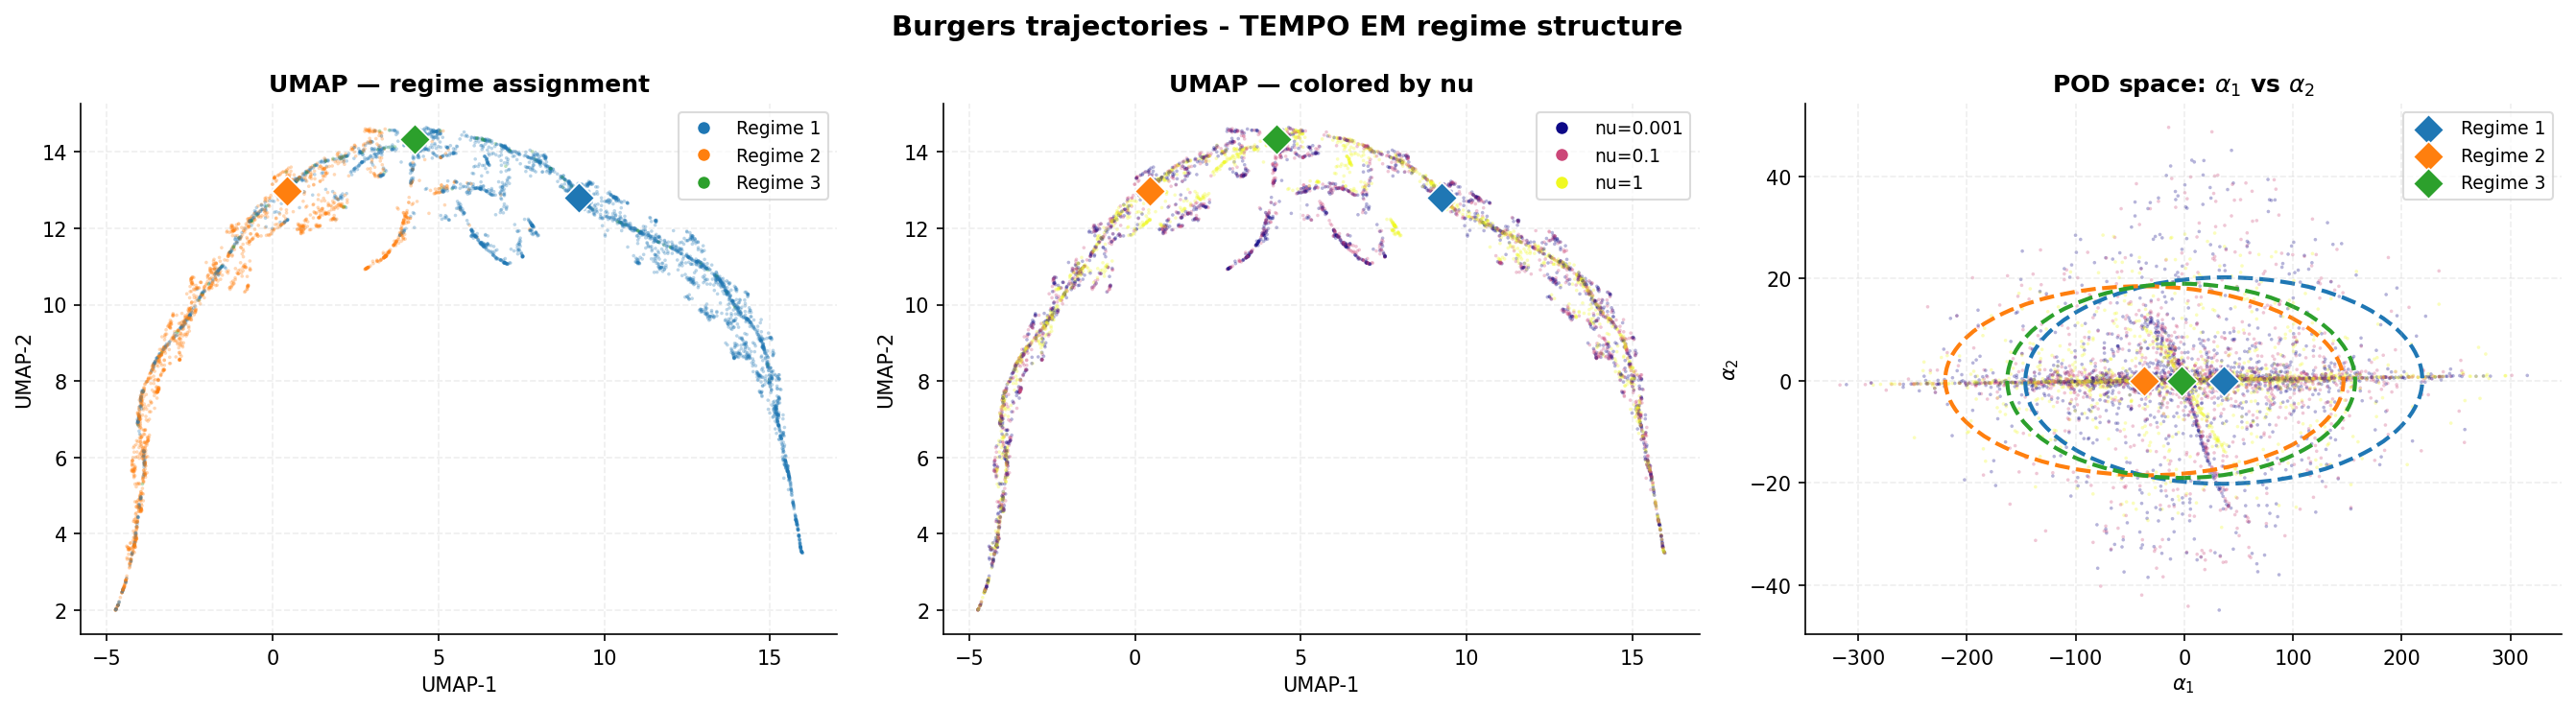
\includegraphics[width=\textwidth]{figs/TEMPO_phase1_burgers_pod_M3.png}
\caption{TEMPO(POD) regime structure on 1D Burgers' ($M{=}3$, 20 EM iterations).
  \textit{Left:} UMAP colored by regime.
  \textit{Center:} same embedding colored by~$\nu$.
  \textit{Right:} GMM fit in POD coefficient space $(\alpha_1,\alpha_2)$;
  stars mark regime centroids~$\mu_m$.}
\label{fig:umap_em}
\end{figure}

Each regime corresponds to a geometric type of initial condition~$u_0$
that appears across all viscosity values.
The per-viscosity gating weights
(Table~\ref{tab:gating}, Appendix~\ref{app:exp}) are nearly uniform across
$\nu\in\{0.001,0.1,1.0\}$, closely matching the global weights
$\boldsymbol{\pi}{=}(0.324,\,0.267,\,0.409)$: regime membership correlates
with initial-condition geometry across all viscosity values.
Within each regime,~$\nu$ shapes the dynamics: the same initial geometry
yields a shock at $\nu{=}0.001$ and a smooth wave at $\nu{=}1.0$.
At inference,~$\nu$ is passed to the branch network as a conditioning input.

%==========================================================================
\subsection{Role of the Physical Parameter}\label{sec:kappa_abl}
%==========================================================================

We ablate the effect of $\kappa$ at inference by replacing it with zero or a learned prediction.
On Burgers', TEMPO(NeuralPOD) barely needs $\kappa$: removing it costs only $1$--$3\%$ in L2, since $u_0$ alone carries enough information to route inputs, consistent with regimes being defined by initial-condition shape.
TEMPO(POD) is more sensitive ($+37\%$); however, $\nu$ can be predicted from $u_0$ with $87\%$ accuracy, reducing the gap to $+7\%$.
On Darcy, $\kappa$ is essential: removing $\beta$ collapses gating to a fixed mixture and increases error by $2$--$3\times$; $\beta$ cannot be predicted from the permeability field $a(x)$ because it is drawn independently in the dataset (classifier accuracy $21\%$, below chance).
Full results are in Table~\ref{tab:kappa_abl} (Appendix~\ref{app:kappa_abl}).

\section{Conclusion}

Operator learning for parametric PDEs typically relies on a single global representation.
When the governing parameter drives qualitative change in solution structure, a single global basis cannot fit all regimes well and prediction quality suffers.

TEMPO discovers regime structure from unlabelled snapshots via EM and fits a dedicated basis to each regime.
The discovered partition captures both sources of solution variability: on 1D Burgers', regimes group solutions by the shape of the initial condition across all viscosity values, while viscosity shapes the dynamics within each regime.
The same initial condition produces a shock at $\nu{=}0.001$ and a smooth wave at $\nu{=}1.0$, yet belongs to the same regime throughout.
A global model conflates these two sources of variation; TEMPO separates them without supervision.

TEMPO(POD) outperforms the joint POD-DeepONet baseline by 13--50\% on Burgers' and up to $5\times$ on Darcy flow, where per-parameter specialists fail catastrophically out-of-distribution.
On Navier-Stokes, TEMPO matches the POD baseline.
TEMPO(NeuralPOD) extends the framework to nonlinear bases; closing the gap with TEMPO(POD) remains an open direction.

Several directions remain open.
Conditioning basis functions on $\kappa$ would let each mode encode parameter-dependent dynamics directly.
Extending regime discovery to continuous parameter spaces and three-dimensional problems is a natural next step.


\clearpage

\bibliographystyle{elsarticle-num}
\bibliography{references}


\newpage
\appendix
\section{Appendix}\label{app}

\subsection{Proof of Proposition~\ref{prop:advantage}}\label{app:proof}

\begin{lemma}\label{lem:mean}
Let $\bar{s}=\tfrac{1}{N}\sum_i s^{(i)}$ be the global mean and
$\bar{s}_m=\tfrac{1}{N_m}\sum_i\gamma_{im}s^{(i)}$ the regime-$m$ mean,
with $N_m=\sum_i\gamma_{im}$.
For any rank-$K$ orthoprojector $P$ and any regime $m$,
\[
  \sum_i \gamma_{im}\|(I{-}P)(s^{(i)}{-}\bar{s}_m)\|_w^2
  =
  \sum_i \gamma_{im}\|(I{-}P)(s^{(i)}{-}\bar{s})\|_w^2
  - N_m\|(I{-}P)(\bar{s}_m{-}\bar{s})\|_w^2.
\]
\end{lemma}
\begin{proof}
Let $c_m=\bar{s}_m-\bar{s}$.
Writing $(I{-}P)(s^{(i)}{-}\bar{s}_m)=(I{-}P)(s^{(i)}{-}\bar{s})-(I{-}P)c_m$
and expanding $\|a-b\|_w^2=\|a\|_w^2-2\langle a,b\rangle_w+\|b\|_w^2$,
then summing over $i$ with weights $\gamma_{im}$:
\begin{align*}
  \sum_i\gamma_{im}\|(I{-}P)(s^{(i)}{-}\bar{s}_m)\|_w^2
  &= \sum_i\gamma_{im}\|(I{-}P)(s^{(i)}{-}\bar{s})\|_w^2 \\
  &\quad -\;2\Bigl\langle(I{-}P)\!\sum_i\gamma_{im}(s^{(i)}{-}\bar{s}),\;(I{-}P)c_m\Bigr\rangle_w \\
  &\quad +\;N_m\|(I{-}P)c_m\|_w^2.
\end{align*}
Since $\sum_i\gamma_{im}(s^{(i)}{-}\bar{s})=N_mc_m$, the cross-term equals
$-2N_m\|(I{-}P)c_m\|_w^2$; together with the quadratic term this gives
$-N_m\|(I{-}P)c_m\|_w^2 = -N_m\|(I{-}P)(\bar{s}_m{-}\bar{s})\|_w^2$.
\end{proof}

\begin{proof}[Proof of Proposition~\ref{prop:advantage}]
Let $P^*$ and $P_m^*$ be the globally and regime-$m$ optimal rank-$K$ projectors.
Since $P_m^*$ minimizes the regime-$m$ objective over all rank-$K$ projectors,
substituting the (generally suboptimal) $P^*$ cannot decrease it:
\[
  \varepsilon_{\mathrm{TEMPO}}^K
  = \sum_m\sum_i\gamma_{im}\|(I{-}P_m^*)(s^{(i)}{-}\bar{s}_m)\|_w^2
  \;\leq\;
  \sum_m\sum_i\gamma_{im}\|(I{-}P^*)(s^{(i)}{-}\bar{s}_m)\|_w^2.
\]
Applying Lemma~\ref{lem:mean} to each $m$ and summing over $m$,
then using $\sum_m\gamma_{im}=1$ for each $i$:
\begin{align*}
  \sum_m\sum_i\gamma_{im}\|(I{-}P^*)(s^{(i)}{-}\bar{s}_m)\|_w^2
  &= \sum_i\|(I{-}P^*)(s^{(i)}{-}\bar{s})\|_w^2
    - \underbrace{\sum_m N_m\|(I{-}P^*)(\bar{s}_m{-}\bar{s})\|_w^2}_{\geq\,0}\\
  &\leq \sum_i\|(I{-}P^*)(s^{(i)}{-}\bar{s})\|_w^2
    = \varepsilon_{\mathrm{global}}^K.
\end{align*}
\end{proof}

\subsection{2D Navier-Stokes Data Generation}\label{app:ns_data}

We use the same equation and forcing as~\citet{Li2021} with a
pseudo-spectral solver in stream-function formulation: diffusion treated
implicitly (Crank--Nicolson), advection explicitly (second-order
Adams--Bashforth), and $\tfrac{2}{3}$-rule dealiasing on the $64{\times}64$
grid. Simulation time-step $\delta t{=}0.01$; each recorded snapshot
aggregates $10$ sub-steps ($\Delta t{=}0.1$). Initial vorticity fields are
random sums of sinusoids,
\[
  \omega_0(\mathbf{x}) = \sum_{k=1}^{7}\frac{a_k}{1{+}k}
  \bigl[\sin(2\pi k\,x_1+\phi_k)+\cos(2\pi k\,x_2+\phi_k)\bigr],
  \quad a_k\sim\mathcal{N}(0,1),\;\phi_k\sim\mathcal{U}[0,2\pi].
\]
A $5\,\mathrm{s}$ burn-in (500 simulation steps) discards transient
behavior before recording begins.

\clearpage
\subsection{Additional Experiments}\label{app:exp}

\paragraph{Regime model selection (1D Burgers')}
Table~\ref{tab:regime_selection} reports BIC, mean assignment entropy~$H$,
and mean test error~$\bar{\varepsilon}$ for $M\in\{2,3,4\}$.
Table~\ref{tab:gating} shows the per-viscosity EM responsibilities alongside
global mixture weights~$\pi_m$.

\begin{table}[h]
\centering
\small
\setlength{\tabcolsep}{12pt}
\caption{Regime count selection on 1D Burgers'.
  BIC $= {-2\log\mathcal{L} + k\log N}$ (lower is better; penalizes complexity);
  $H$: mean assignment entropy (higher gain signals a new genuine regime);
  $\bar{\varepsilon}$: mean relative $L^2$ test error.
  BIC increases monotonically, favoring $M{=}2$ by complexity alone.
  \textbf{Bold row}: selected configuration ($M{=}3$), chosen because the entropy
  gain $\Delta H{=}0.30$ from $M{=}2{\to}3$ substantially exceeds $\Delta H{=}0.18$
  from $M{=}3{\to}4$.}
\label{tab:regime_selection}
\begin{tabular}{c c c c}
\toprule
$M$ & BIC (${\times}10^{4}$, $\downarrow$) & $H$ & $\bar{\varepsilon}$ \\
\midrule
2          & 3.90 & 0.622 & 0.209 \\
\textbf{3} & \textbf{4.92} & \textbf{0.920} & 0.222 \\
4          & 5.47 & 1.099 & 0.228 \\
\bottomrule
\end{tabular}
\end{table}

\begin{table}[h]
\centering
\small
\setlength{\tabcolsep}{14pt}
\caption{Mean EM assignment weights per viscosity (1D Burgers',
  TEMPO(POD), $M{=}3$) vs.\ global mixture weights~$\pi_m$.
  Each row sums to~$1$.}
\label{tab:gating}
\begin{tabular}{c c c c}
\toprule
$\nu$ & Regime~1 & Regime~2 & Regime~3 \\
\midrule
0.001 & 0.32 & 0.28 & 0.40 \\
0.1   & 0.32 & 0.26 & 0.42 \\
1.0   & 0.33 & 0.26 & 0.41 \\
\midrule
$\pi_m$ & 0.32 & 0.27 & 0.41 \\
\bottomrule
\end{tabular}
\end{table}

\paragraph{Role of the physical parameter (ablation)}\label{app:kappa_abl}
Table~\ref{tab:kappa_abl} reports the effect of replacing $\kappa$ with zero or a learned prediction at inference.

\begin{table}[h]
\centering
\small
\setlength{\tabcolsep}{6pt}
\caption{$\kappa$ ablation: increase in mean relative L2 error when $\kappa$ is removed or predicted, relative to the real-$\kappa$ baseline.
  For Darcy, $\beta$ is drawn independently of $a(x)$; prediction from input data is not possible.}
\label{tab:kappa_abl}
\begin{tabular}{l c c c c}
\toprule
 & \multicolumn{2}{c}{Burgers'} & \multicolumn{2}{c}{Darcy} \\
\cmidrule(lr){2-3}\cmidrule(lr){4-5}
 & NeuralPOD ($M{=}3$) & POD ($M{=}3$) & NeuralPOD ($M{=}5$) & POD ($M{=}5$) \\
\midrule
$\kappa = 0$ & $+0.006$ ($+1\%$) & $+0.127$ ($+37\%$) & $+0.334$ ($+27\%$) & $+0.618$ ($+219\%$) \\
$\kappa$ predicted from $u_0$ & \textemdash & $+0.024$ ($+7\%$) & \multicolumn{2}{c}{not predictable} \\
\bottomrule
\end{tabular}
\end{table}

\paragraph{POD vs.\ NeuralPOD basis comparison (1D Burgers')}
Figure~\ref{fig:basis_spectrum} shows the singular-value and residual decay for POD ($K{=}30$ modes capture $99.99\%$ of the variance) and Fourier NeuralPOD.
The corresponding spatiotemporal mode functions (Figure~\ref{fig:basis_modes_collage}) reveal a structural difference: POD modes are globally supported, while NeuralPOD modes localise adaptively — at $\nu{=}0.01$ they concentrate near the shock front.
Per-sample reconstructions from both bases are compared in Figure~\ref{fig:basis_reconstruction}; additional NeuralPOD examples are shown in Figure~\ref{fig:basis_rec}.

\begin{figure}[!htbp]
\centering

\includegraphics[width=\textwidth]{TEMPO/main/figs/basis_spectrum_nu1.0.png}
\caption{Basis convergence on 1D Burgers' ($\nu{=}1.0$): POD singular-value decay (\textit{left}); Fourier NeuralPOD residual decay (\textit{right}).}
\label{fig:basis_spectrum}
\end{figure}

\begin{figure}[!htbp]
\centering
\begin{subfigure}{\textwidth}
  \centering
  
\includegraphics[width=0.9\textwidth]{TEMPO/main/figs/basis_modes_nu1.0.png}
  \caption{$\nu{=}1.0$}
  \label{fig:basis_modes}
\end{subfigure}
\\[0.5ex]
\begin{subfigure}{\textwidth}
  \centering
  
\includegraphics[width=0.9\textwidth]{TEMPO/main/figs/basis_modes_nu0.01.png}
  \caption{$\nu{=}0.01$}
  \label{fig:basis_modes_nu001}
\end{subfigure}
\caption{First $K$ basis modes on 1D Burgers': POD (\textit{top row}) vs.\ Fourier NeuralPOD (\textit{bottom row}).}
\label{fig:basis_modes_collage}
\end{figure}

\begin{figure}[!htbp]
\centering

\includegraphics[width=0.85\textwidth]{TEMPO/main/pictures/Neural_POD_rec_basis.png}
\caption{Fourier NeuralPOD representative reconstructions on 1D Burgers' ($\nu{=}1.0$).}
\label{fig:basis_rec}
\end{figure}


\begin{figure}[!htbp]
\centering

\includegraphics[width=\textwidth]{TEMPO/main/figs/basis_reconstruction_nu1.0.png}
\caption{Phase~1 reconstruction comparison on 1D Burgers' ($\nu{=}1.0$).
  Each row shows one sample: ground truth, POD reconstruction, $|$POD error$|$,
  Fourier NeuralPOD reconstruction, $|$FNPOD error$|$.}
\label{fig:basis_reconstruction}
\end{figure}


\paragraph{Representative reconstructions (1D Burgers')}
Figure~\ref{fig:burgers_rec_collage} shows space--time predictions for all four methods on 1D Burgers' ($\nu{=}1.0$). Each panel: ground truth (\textit{left}), prediction (\textit{center}), point-wise error (\textit{right}).

\begin{figure}[!htbp]
\centering
\begin{subfigure}[t]{0.48\textwidth}
  \centering
  
\includegraphics[width=\textwidth]{TEMPO/main/pictures/pod_reconstruction.png}
  \caption{POD-DeepONet}
  \label{fig:pod_reconstruction}
\end{subfigure}
\hfill
\begin{subfigure}[t]{0.48\textwidth}
  \centering
  
\includegraphics[width=\textwidth]{TEMPO/main/pictures/npod_reconstruction.png}
  \caption{NeuralPOD-DeepONet}
  \label{fig:npod_reconstruction}
\end{subfigure}
\\[1ex]
\begin{subfigure}[t]{0.48\textwidth}
  \centering
  
\includegraphics[width=\textwidth]{TEMPO/main/figs/tempo_pod_burgers_reconstruct.png}
  \caption{TEMPO(POD), $M{=}3$}
  \label{fig:tempo_pod_burgers_rec}
\end{subfigure}
\hfill
\begin{subfigure}[t]{0.48\textwidth}
  \centering
  
\includegraphics[width=\textwidth]{TEMPO/main/figs/tempo_npod_burgers_reconstruct.png}
  \caption{TEMPO(NeuralPOD), $M{=}3$: high-frequency noise (L2 $0.46$--$0.54$)}
  \label{fig:tempo_npod_burgers_rec}
\end{subfigure}
\caption{Space--time reconstructions on 1D Burgers' ($\nu{=}1.0$).}
\label{fig:burgers_rec_collage}
\end{figure}

\paragraph{TEMPO regime structure across benchmarks}
Figure~\ref{fig:umap_all} compares the Phase~1 regime structure across all three benchmarks.
On Burgers' (NeuralPOD), the partition mirrors the POD variant (Figure~\ref{fig:umap_em}) with sharper assignments.
On Darcy flow, regimes span multiple $\beta$ values; TEMPO(NeuralPOD) finds a nearly identical partition.
On Navier-Stokes, all Re values overlap in POD coefficient space and regimes 2--4 collapse to a few points, explaining why dedicated bases bring no gain.

\begin{figure}[!htbp]
\centering
\begin{subfigure}{\textwidth}
  \centering
  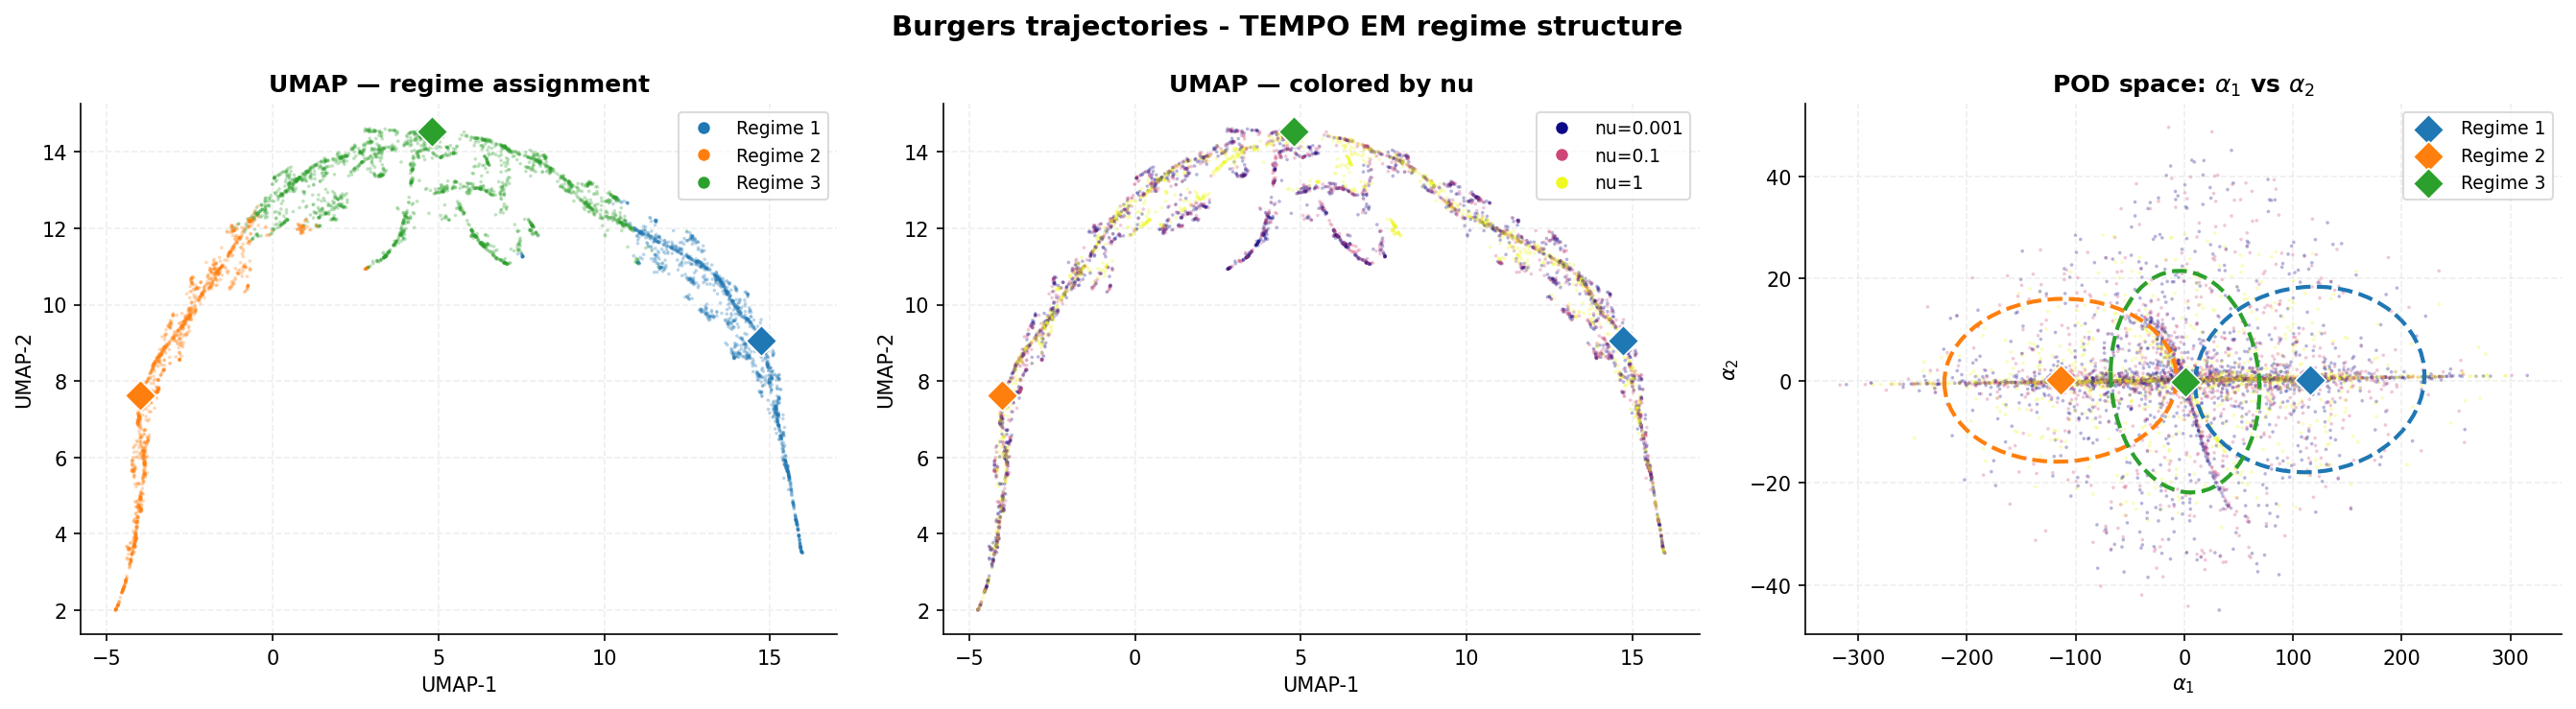
\includegraphics[width=0.85\textwidth]{figs/TEMPO_phase1_burgers_npod_M3.png}
  \caption{1D Burgers', NeuralPOD ($M{=}3$, $H{=}0.23$)}
  \label{fig:umap_em_npod}
\end{subfigure}
\\[0.5ex]
\begin{subfigure}{\textwidth}
  \centering
  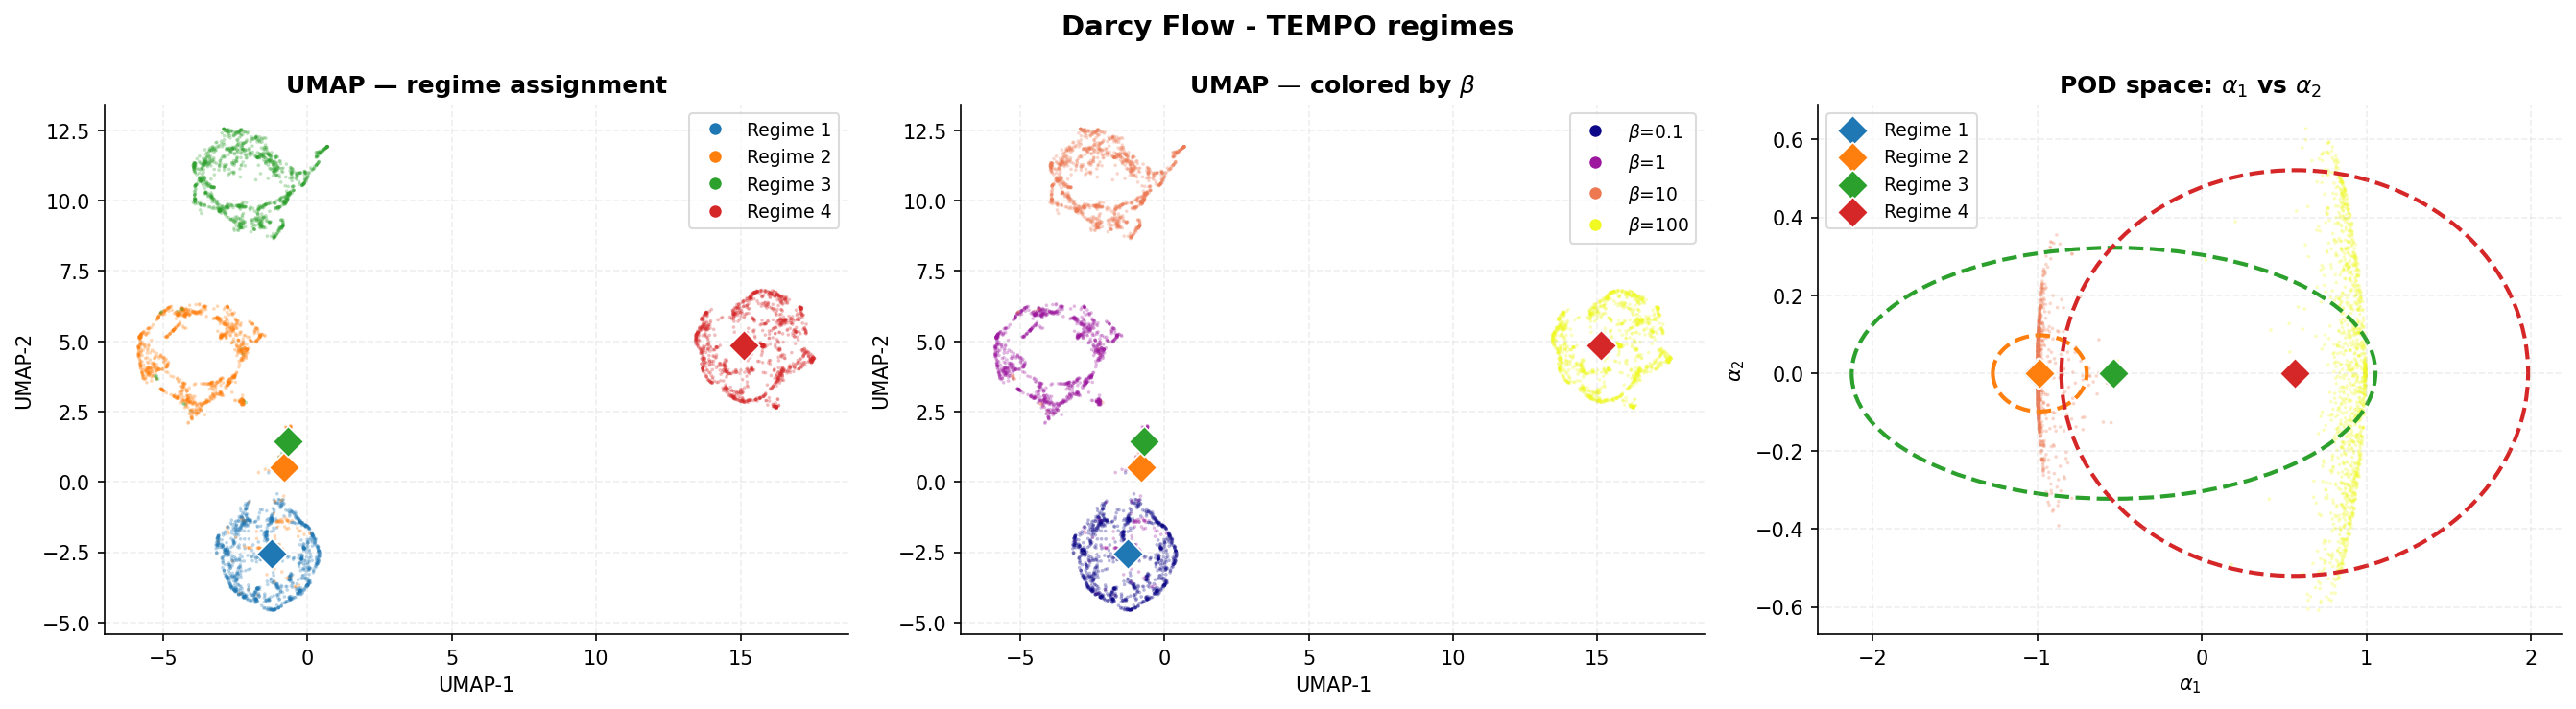
\includegraphics[width=0.85\textwidth]{figs/TEMPO_phase1_darcy_pod_M4.png}
  \caption{2D Darcy flow, POD ($M{=}4$)}
  \label{fig:tempo_phase1_darcy}
\end{subfigure}
\\[0.5ex]
\begin{subfigure}{\textwidth}
  \centering
  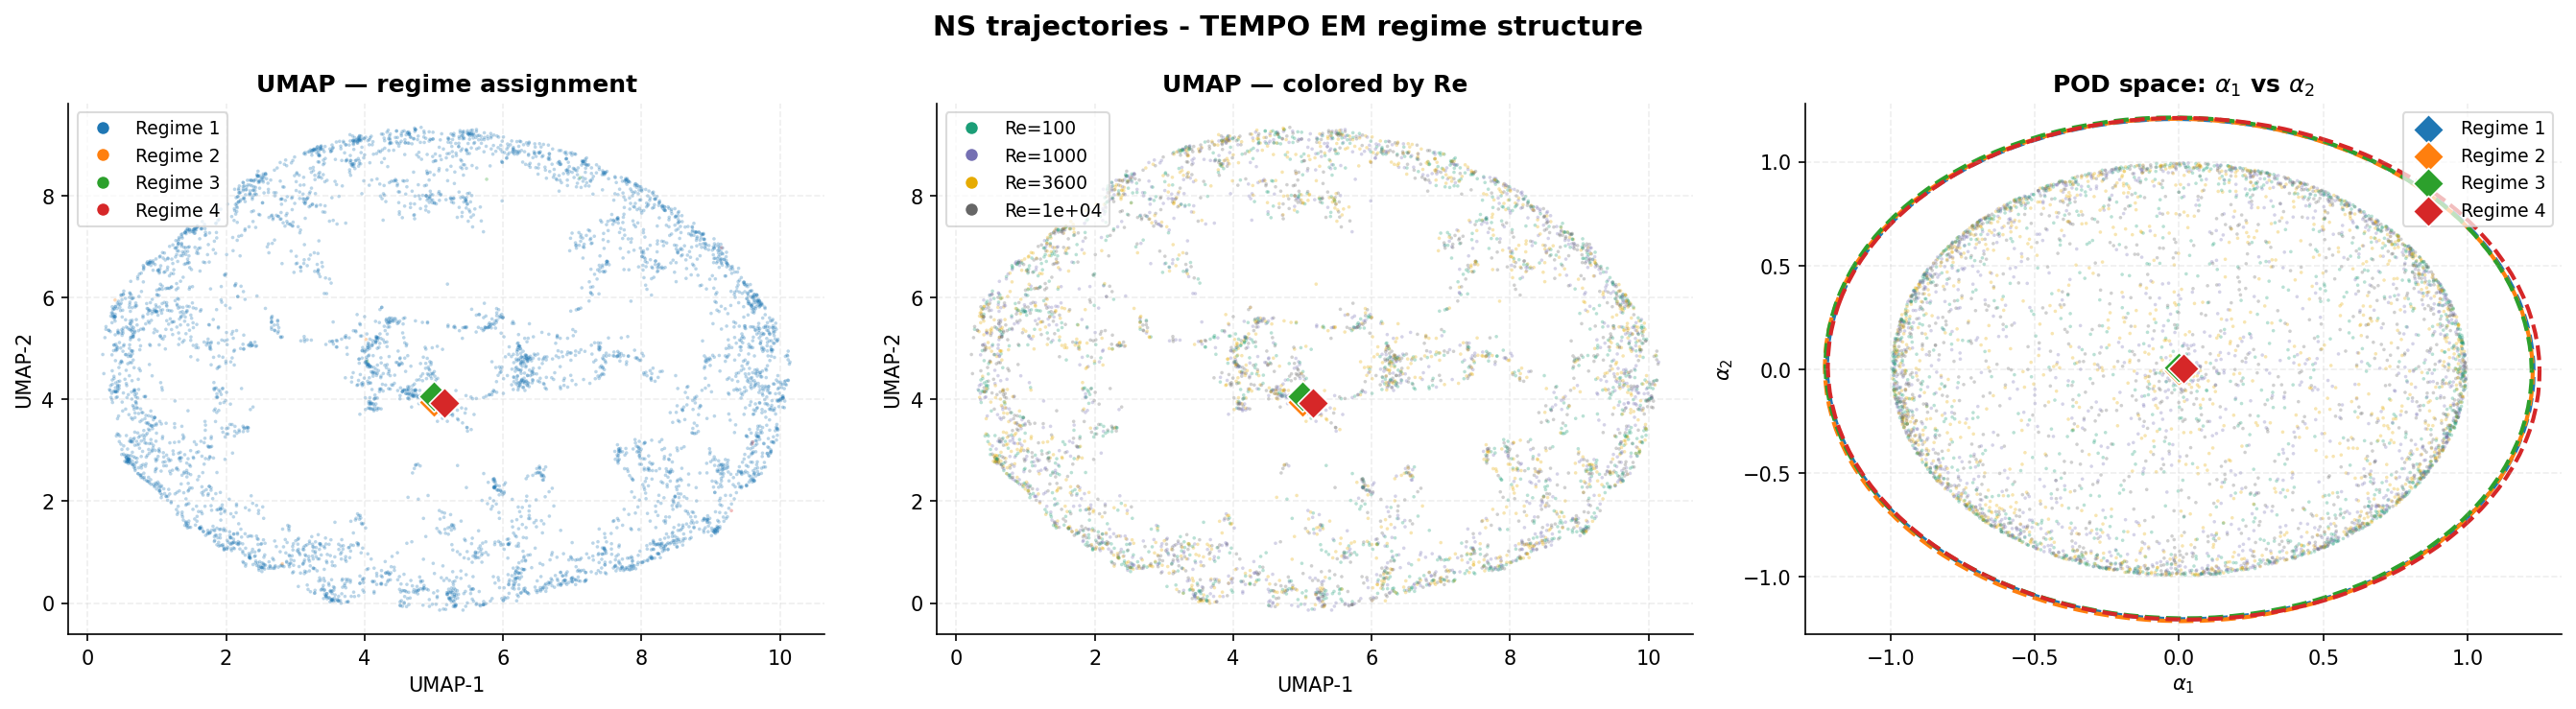
\includegraphics[width=0.85\textwidth]{figs/ns_tempo_phase1.png}
  \caption{2D Navier-Stokes, POD ($M{=}4$): no Re separation}
  \label{fig:ns_tempo_phase1}
\end{subfigure}
\caption{TEMPO EM regime structure across all benchmarks. Layout as in Figure~\ref{fig:umap_em}.}
\label{fig:umap_all}
\end{figure}

\paragraph{TEMPO reconstructions (2D Darcy flow)}
Figure~\ref{fig:darcy_rec_collage} shows representative predictions from both TEMPO variants on 2D Darcy flow ($M{=}5$). Each panel: ground truth (\textit{left}), prediction (\textit{center}), point-wise error (\textit{right}).

\begin{figure}[!htbp]
\centering
\begin{subfigure}[t]{0.44\textwidth}
  \centering
  
\includegraphics[width=\textwidth]{TEMPO/main/figs/tempo_pod_darcy_reconstruct.png}
  \caption{TEMPO(POD)}
  \label{fig:tempo_pod_darcy_rec}
\end{subfigure}
\hspace{0.04\textwidth}
\begin{subfigure}[t]{0.44\textwidth}
  \centering
  
\includegraphics[width=\textwidth]{TEMPO/main/figs/tempo_npod_darcy_reconstruct.png}
  \caption{TEMPO(NeuralPOD)}
  \label{fig:tempo_npod_darcy_rec}
\end{subfigure}
\caption{Space--time reconstructions on 2D Darcy flow ($M{=}5$).}
\label{fig:darcy_rec_collage}
\end{figure}

\paragraph{TEMPO reconstructions (2D Navier-Stokes)}
Figure~\ref{fig:ns_rec_collage} shows representative predictions from TEMPO(POD) and TEMPO(NeuralPOD) on 2D Navier-Stokes ($M{=}4$); EM convergence is shown in Figure~\ref{fig:ns_em_convergence}.

\begin{figure}[!htbp]
\centering
\begin{subfigure}{\textwidth}
  \centering
  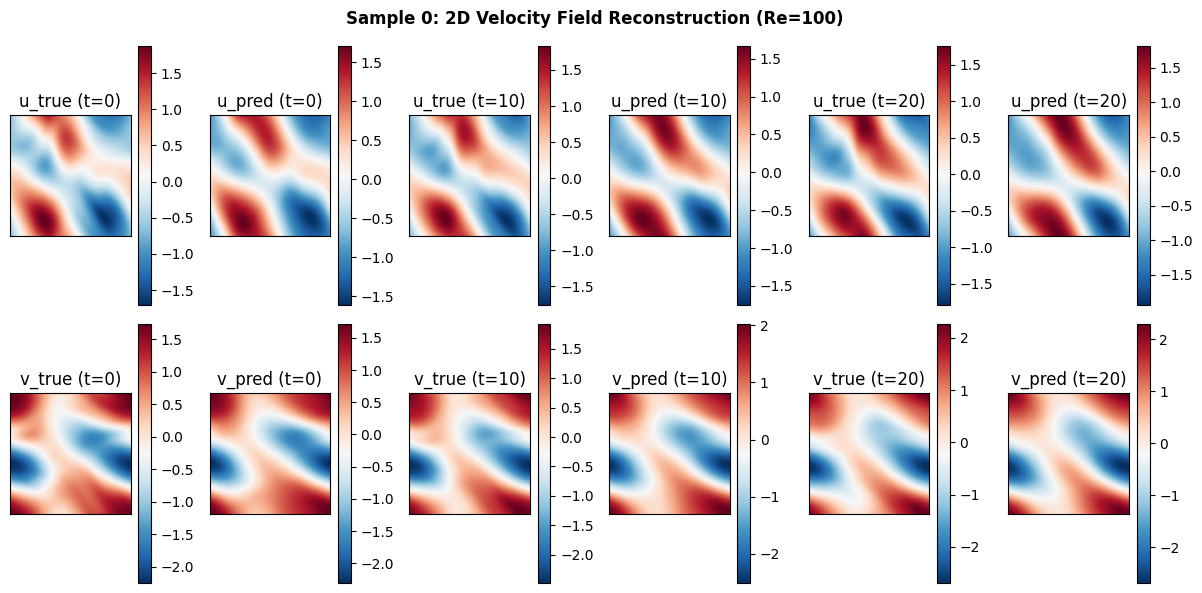
\includegraphics[width=0.88\textwidth]{figs/ns_reconstruction_sample0.png}
  \caption{TEMPO(POD): ground truth (\textit{left}), prediction (\textit{center}), point-wise absolute error (\textit{right}).}
  \label{fig:ns_reconstruction}
\end{subfigure}
\\[0.3ex]
\begin{subfigure}{\textwidth}
  \centering
  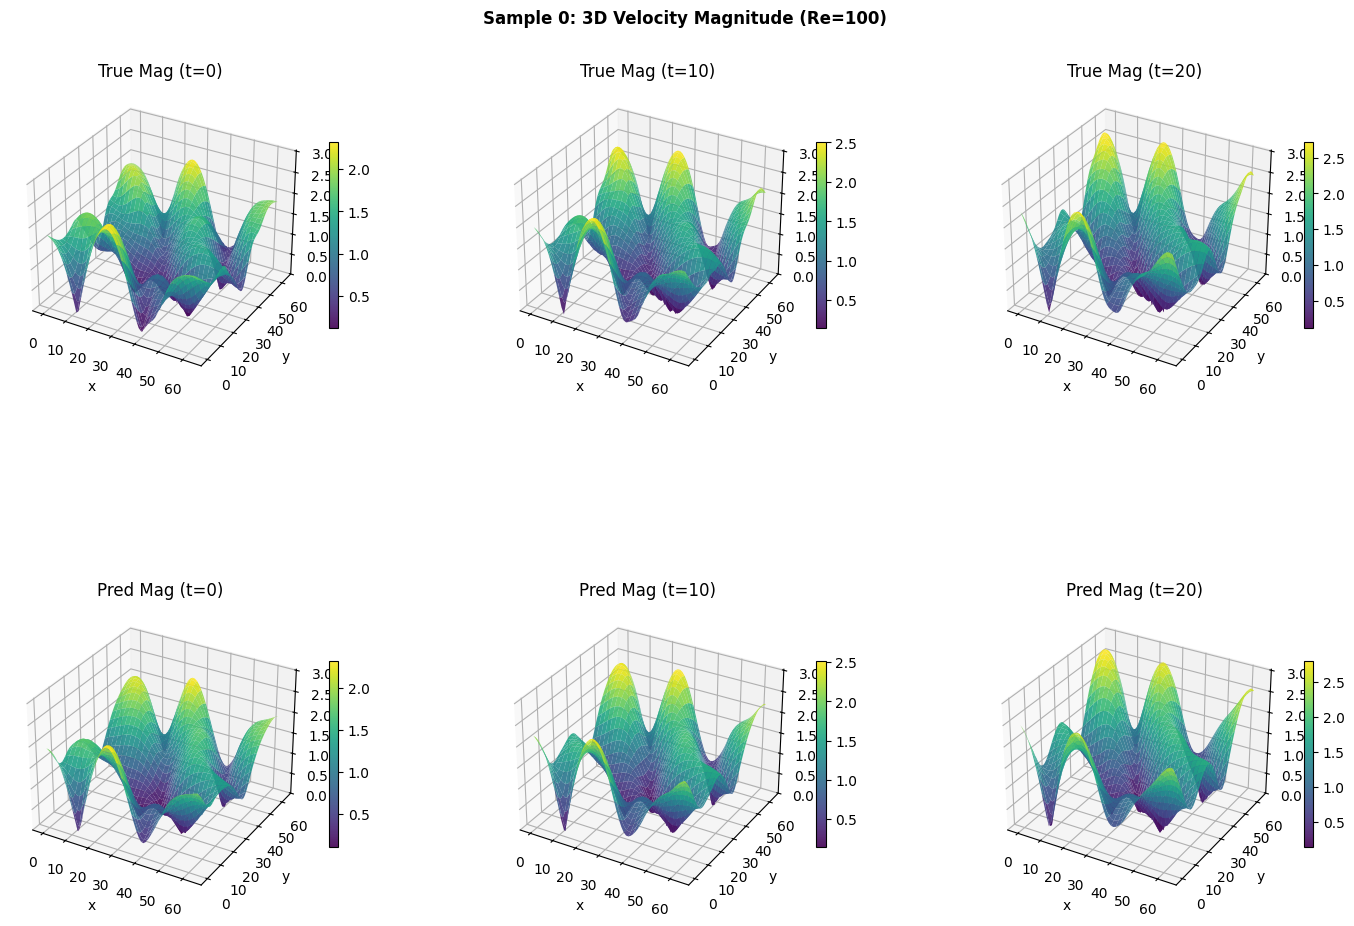
\includegraphics[width=0.62\textwidth]{figs/ns_reconstruction_3d_sample0.png}
  \caption{TEMPO(POD) — 3D vorticity field.}
  \label{fig:ns_reconstruction_3d}
\end{subfigure}
\\[0.3ex]
\begin{subfigure}{\textwidth}
  \centering
  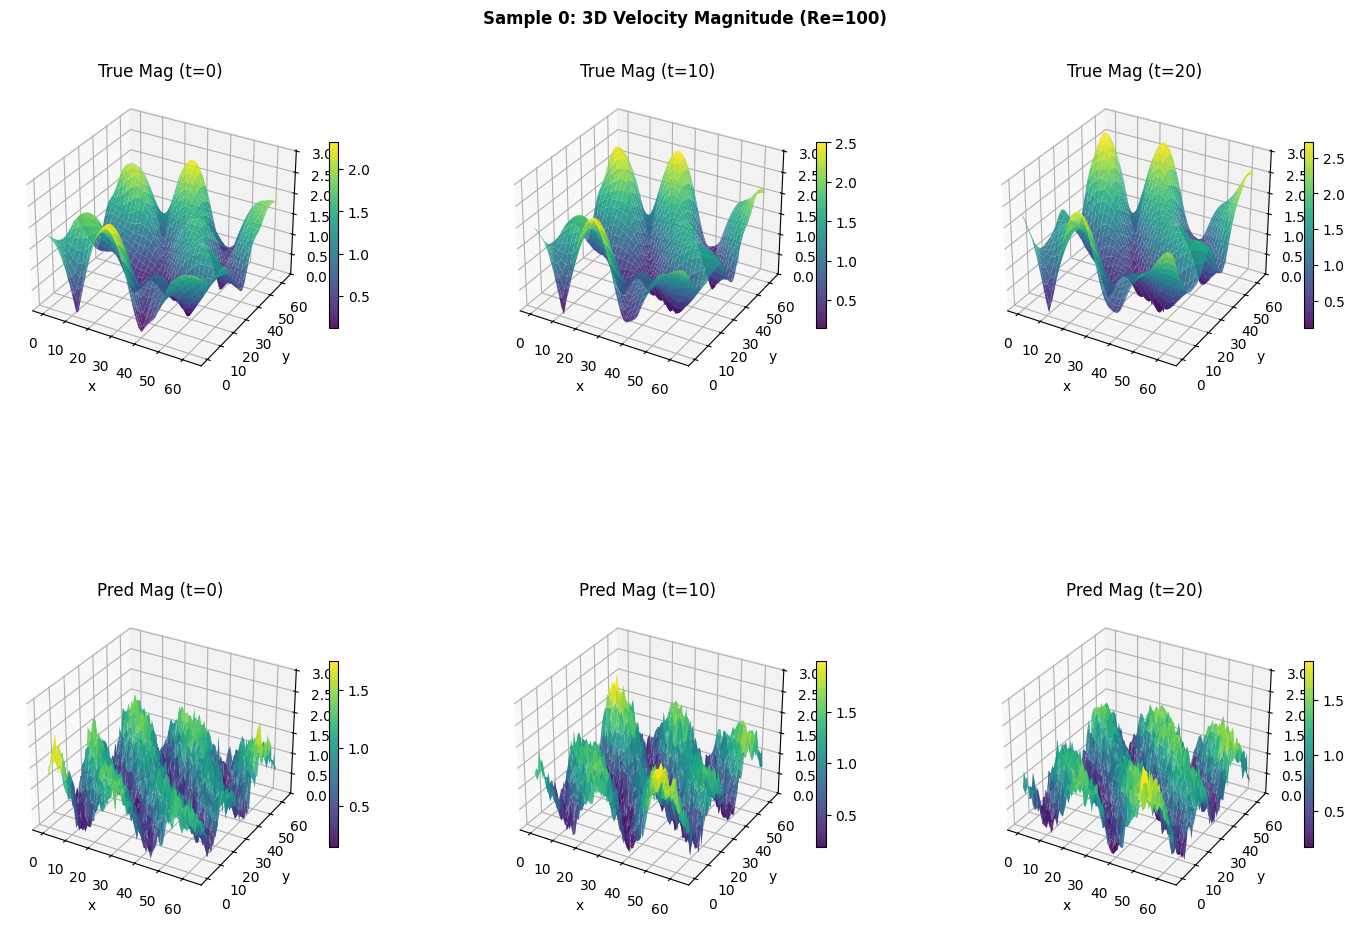
\includegraphics[width=0.62\textwidth]{figs/tempo_npod_ns_reconstruction_3d_sample0.png}
  \caption{TEMPO(NeuralPOD) — 3D vorticity field.}
  \label{fig:ns_npod_reconstruction_3d}
\end{subfigure}
\caption{2D Navier-Stokes ($M{=}4$): TEMPO(POD) prediction (\textit{top}); TEMPO(POD) and TEMPO(NeuralPOD) 3D vorticity (\textit{middle}, \textit{bottom}).}
\label{fig:ns_rec_collage}
\end{figure}

\begin{figure}[!htbp]
\centering
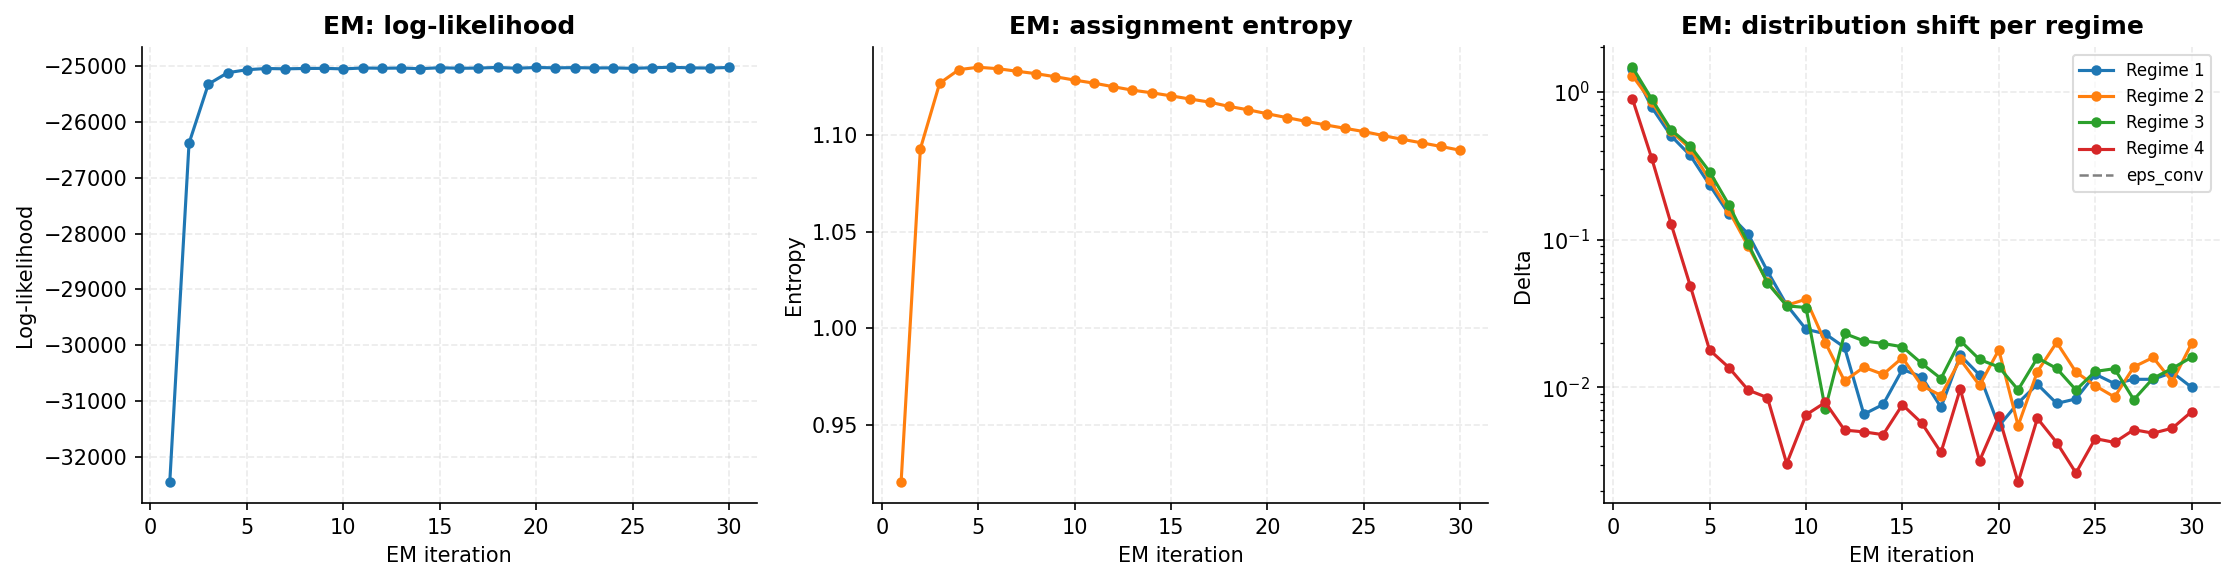
\includegraphics[width=\textwidth]{figs/ns_em_convergence.png}
\caption{TEMPO(POD) EM convergence on 2D Navier-Stokes ($M{=}4$).}
\label{fig:ns_em_convergence}
\end{figure}

\subsection{Algorithms}\label{app:alg}

\begin{algorithm}[H]
\caption{\textsc{NeuralBasis}}
\label{alg:npod}
\begin{algorithmic}[1]
\Require weighted snapshots $\{s^{(i)},\,\gamma_{im}\}_{i=1}^N$, tolerance $\tau$
\Ensure basis $\phi_0^{(m)},\;\bigl\{\phi_k^{(m)},\,\{\lambda_k^{(m,i)}\}_{i=1}^N\bigr\}_{k=1}^{K_m}$
\State $\bar{s}^{(m)} \leftarrow \displaystyle\frac{1}{N_m}\sum_{i=1}^N \gamma_{im}\,s^{(i)},\quad N_m = \sum_{i=1}^N\gamma_{im}$
  \hfill\Comment{responsibility-weighted mean trajectory}
\State Train $\phi_0^{(m)}$ by minimizing
  $\displaystyle\sum_j w_j\bigl(\phi_0^{(m)}(y_j) - \bar{s}^{(m)}_j\bigr)^2$
\State $r^{(0,i)} \leftarrow s^{(i)} - \phi_0^{(m)}(y)$
  \enspace for all $i$;\enspace $k \leftarrow 0$
\State $V_m \leftarrow \displaystyle\sum_{i=1}^N \gamma_{im}\,\|s^{(i)}-\bar{s}^{(m)}\|_w^2$
  \hfill\Comment{initial unmodeled variance}
\While{$\displaystyle\sum_{i=1}^N \gamma_{im}\,\|r^{(k,i)}\|_w^2
  \;\ge\; \tau\, V_m$ \textbf{ and } $k < K_{\max}$}
  \State Jointly minimize over $\phi_{k+1}^{(m)}$ and
    $\{\lambda_{k+1}^{(m,i)}\}_{i=1}^N$:
    \[
      \sum_{i=1}^N \gamma_{im}
      \sum_j w_j\!\left(\lambda_{k+1}^{(m,i)}\,\phi_{k+1}^{(m)}(y_j)
      - r^{(k,i)}_j\right)^{\!2}
    \]
  \State $r^{(k+1,i)} \leftarrow r^{(k,i)}
    - \lambda_{k+1}^{(m,i)}\,\phi_{k+1}^{(m)}(y)$
    \enspace for all $i$
  \State $k \leftarrow k + 1$
\EndWhile
\State \Return $K_m \!\leftarrow\! k$,\enspace
  $\phi_0^{(m)}$,\enspace
  $\bigl\{\phi_k^{(m)},\,\{\lambda_k^{(m,i)}\}_{i=1}^N\bigr\}_{k=1}^{K_m}$
\end{algorithmic}
\end{algorithm}

\begin{algorithm}[H]
\caption{\textsc{TEMPO}}
\label{alg:tempo}
\begin{algorithmic}[1]
\Require $\mathcal{D} = \{u_0^{(i)}, \kappa^{(i)}, s^{(i)}\}_{i=1}^N$;\;
  $M,\;\varepsilon_s,\;\varepsilon_l,\;\varepsilon_p,\;\varepsilon_c,\;\tau$
\Ensure Regime bases $\{\Phi_m^*\}$,\;
  amplitudes $\{\Lambda_m^*\}$,\;
  responsibilities $\{\gamma_{im}^*\}$,\;
  weights $\{\pi_m^*\}$
%
\Statex \textit{Initialization}
\State Compute global POD on $\{s^{(i)}\}$;
  project to $\alpha^{(i)} \in \mathbb{R}^{d_0}$ for all $i$
\State Run GMM-EM on $\{\alpha^{(i)}\}$ $\to$
  $\gamma_{im}^{(0)},\;\pi_m^{(0)},\;\mu_m^{(0)},\;\Sigma_m^{(0)}$
\For{$m = 1,\ldots,M$}
  \State $\Phi_m^{(0)},\,\Lambda_m^{(0)} \leftarrow$
    \Call{NeuralBasis}
    {$\{s^{(i)},\gamma_{im}^{(0)}\},\,\tau$}
    \hfill\Comment{or weighted SVD for TEMPO(POD), see \S\ref{sec:bases}}
\EndFor
\State $\sigma^2 \leftarrow (2N)^{-1}\!\sum_{i,m}
  \gamma_{im}^{(0)}\,\|s^{(i)}{-}\hat{s}_m^{(i)}\|_w^2$
  \hfill\eqref{eq:sigma2_calib}
%
\Statex \textit{EM iterations}
\Repeat
  \Statex \quad\textit{E-step}
  \For{all $i = 1,\ldots,N$ and $m = 1,\ldots,M$}
    \State Compute $\hat{s}_m^{(i)}$ via~\eqref{eq:separable}
      using $\Phi_m^{(q-1)}$ and $\Lambda_m^{(q-1)}$
    \State $\gamma_{im}^{(q)} \leftarrow$ Eq.~\eqref{eq:estep}
  \EndFor
  \Statex \quad\textit{M-step: mixture weights}
  \State $\pi_m^{(q)} \leftarrow N_m^{(q)}/N$
    for all $m$ \hfill\eqref{eq:mstep_pi}
  \Statex \quad\textit{M-step: bases}
  \For{$m = 1,\ldots,M$}
    \State Compute $\mu_m^{(q)}$~\eqref{eq:mu},\;
      $\Sigma_m^{(q)}$~\eqref{eq:Sigma},\;
      $\Delta_m^{(q)}$~\eqref{eq:Delta}
    \If{$\Delta_m^{(q)} < \varepsilon_s$}
      \State $\Phi_m^{(q)} \leftarrow \Phi_m^{(q-1)}$
        \hfill \textsc{Skip}
    \ElsIf{$\Delta_m^{(q)} < \varepsilon_l$}
      \hfill \textsc{Incremental}
      \State Compute $r_m^{(K_m)}$ under updated $\gamma^{(q)}$;\;
        $V_m^{(q)} \leftarrow \sum_i\gamma_{im}^{(q)}\|s^{(i)}{-}\bar{s}_m^{(q)}\|_w^2$
      \If{$\sum_i\gamma_{im}^{(q)}\|r_m^{(K_m,i)}\|_w^2 \ge \tau\cdot V_m^{(q)}$}
        \State Train mode $K_m{+}1$;\; $K_m \leftarrow K_m + 1$
      \EndIf
      \If{$\|\phi_{K_m}^{(m)}\|_w^2\cdot\displaystyle\sum_{i=1}^N
        \gamma_{im}^{(q)}\,\bigl(\lambda_{K_m}^{(m,i)}\bigr)^2 < \varepsilon_p$}
        \State $K_m \leftarrow K_m - 1$
      \EndIf
    \Else
      \hfill \textsc{Full rerun}
      \State $\Phi_m^{(q)},\,\Lambda_m^{(q)} \leftarrow$
        \Call{NeuralBasis}
        {$\{s^{(i)},\gamma_{im}^{(q)}\},\,\tau$}
    \EndIf
  \EndFor
\Until{$\max_m \Delta_m^{(q)} < \varepsilon_c$}
\State \Return $\Phi_m^* \!\leftarrow\! \Phi_m^{(q)}$,\;
  $\Lambda_m^* \!\leftarrow\! \Lambda_m^{(q)}$,\;
  $\gamma_{im}^* \!\leftarrow\! \gamma_{im}^{(q)}$,\;
  $\pi_m^* \!\leftarrow\! \pi_m^{(q)}$
\end{algorithmic}
\end{algorithm}

\end{document}